\documentclass[12pt]{article}

\usepackage{lineno,hyperref}
\pdfoutput=1
%\usepackage{cite}
\usepackage{graphics}
\usepackage[english] {babel}
\usepackage{amssymb,amsfonts,amsmath,mathtext}
\usepackage{graphicx}
%\usepackage{longtable}
\usepackage{xcolor}
\usepackage{pict2e}
%\usepackage{subcaption}
%\captionsetup[subfigure]{justification=justified,singlelinecheck=false}
%\usepackage{tablefootnote}
%\pagestyle{empty}

\usepackage{subfig}
\usepackage{floatrow}
\usepackage{nicefrac}
%
\usepackage{float}
\floatstyle{plaintop}
\restylefloat{table}

\usepackage{natbib}
\bibliographystyle{abbrvnat}
\setcitestyle{authoryear,open={(},close={)}}

\interfootnotelinepenalty=10000

\renewcommand{\baselinestretch}{1.2}
\renewcommand{\figurename}{Figure}
%\newcommand{\Ex}{{\mathsf{E}\,}}
\DeclareMathOperator{\Ex}{\mathbb{E}}
\newcommand{\Var}{{\mathsf{Var}}\,}
\newcommand{\R}{{\mathbb R}}
\newcommand{\T}{{\mathbb T}}
\renewcommand{\S}{{\mathbb S}}
\newcommand{\rms}{{\mathsf{rms}}\,}
\newcommand{\supp}{{\mathsf{supp}}\,}
\newcommand{\Corr}{{\mathsf{Corr}}\,}
\newcommand{\Cov}{{\mathsf{Cov}}\,}
\newcommand{\vecg}{{\mathsf{vec}}\,}
%\newcommand{\lik}{{\mathsf{lik}}\,}
\newcommand{\vecs}{{\mathsf{vecs}}\,}
\newcommand{\Med}{{\mathsf{Med}}\,}
\newcommand{\range}{{\mathsf{range}}\,}
\newcommand{\constant}{{\mathsf{const}}}
\newcommand{\cond}{{\mathsf{cond}}\,}
\newcommand{\Ku}{{\mathsf{Ku}}\,}
\newcommand{\diag}{{\mathsf{diag}}}
\newcommand{\sign}{{\mathsf{sign}}}
\DeclareMathOperator*{\argmin}{argmin}
\DeclareMathOperator{\tr}{tr}
\DeclareMathOperator{\sd}{SD}
\DeclareMathOperator{\lik}{lik}
\renewcommand{\d}{{\rm d}}
\renewcommand{\Pr}{{\mathsf{P}\,}}
%\newcommand{\eg}{e.g.\ }
\newcommand{\etc}{etc.\ }
\newcommand{\eg}{e.g.,\ }
%\newcommand{\eeg}{E.g.\ }
\newcommand{\eeg}{E.g.,\ }
\newcommand{\cf}{{\em cf.\ }}
\newcommand{\vs}{vs.\ }
\newcommand{\ie}{i.e., }
\newcommand{\wrt}{w.r.t.\ }
\newcommand{\lhs}{l.h.s.\ }
\newcommand{\rhs}{r.h.s.\ }
\newcommand{\e}{\mathrm{e}}
\renewcommand{\i}{\mathsf{i}}
\def\mymathhyphen{{\hbox{-}}}

\textheight=25.0cm
\textwidth=16.0cm
\topmargin=-1.0in
\setlength{\evensidemargin}{2mm}
\setlength{\oddsidemargin}{2mm}

\newcommand{\green}{\textcolor[rgb]{0,0.8,0.2}}
\newcommand{\blue}{\textcolor[rgb]{0,0,1}}
\newcommand{\red}{\textcolor[rgb]{1,0,0}}

\newcommand{\verde}{\textcolor[rgb]{0,0.8,0.2}}
\newcommand{\blu}{\textcolor[rgb]{0,0,1}}
\newcommand{\rosso}{\textcolor[rgb]{1,0,0}}

\newcommand{\seroburmalin}{\textcolor[rgb]{0.2,0.5,0.3}}
\newcommand{\serobur}{\textcolor[rgb]{0.1,0.35,0.25}}
\newcommand{\orange}{\textcolor[rgb]{1,0.5,0}}
\newcommand{\black}{\textcolor[rgb]{0,0,0}}

\newcommand{\greeen}{\textcolor[rgb]{0.2, 0.9, 0.2}}
\newcommand{\olive}{\textcolor[rgb]{0.3, 0.4, .1}}
\newcommand{\gold}{\textcolor[rgb]{1.0, 0.84, 0.}}


\modulolinenumbers[5]

\bibliographystyle{plain}
\sloppy



   \title{The ensemble Kalman filter regularized with \\non-parametric
   non-stationary spatial convolutions\\
    \bigskip
%    \large{\bf Working paper}
}
   \author{M Tsyrulnikov and A Sotskiy\\
   \smallskip
   {\em HydroMetCenter of Russia}\\
   %{\small (tsyrulnikov@mecom.ru) }
   }


\begin{document}
\maketitle




%-----------------------------------------------------------
\section {Introduction}




Modern  data assimilation increasingly relies on the ensemble technique,
in which the prior probability distribution of the truth is represented by
a finite sample (ensemble) of pseudo-random realizations (called ensemble members).
This allows for realistic spatially varying, flow-dependent prior (forecast-error) covariances in the analysis
(\ie in the observation update step of the data assimilation cycle).
In practical applications, the  most widely used approach is the Ensemble Kalman Filter (EnKF),
which makes use of ensemble (sample) covariances.
The principal problem of the ensemble approach is  that running many ensemble members is
computationally expensive. In real-world very-high-dimensional problems,
this means that only very small ensembles (normally, comprising just tens of members) are affordable.
As a result, such ensembles can  provide the analysis  with
only scarce information on the true prior distribution. The sample covariance matrix 
(a sufficient statistic for the true covariance matrix) is a poor estimate if the sample size
is much lower than the dimensionality if the state space.
As a result, a kind of {\em regularization} (\ie the introduction of
additional information on the prior covariances) is required.






%----------------------------
\subsection {Covariance regularization in EnKF}
\label{sec_covregu}





There exist the following  main practical approaches to  covariance matrix regularization.
%
\begin{enumerate}
\item
The most popular approach is covariance
localization (tapering), \citep[e.g.][]{Houtekamer1998,Furrer},
which reduces spurious long-distance correlations through element-wise multiplication
of the sample covariance matrix by an ad-hoc analytical localization covariance matrix.
This technique efficiently removes a lot of noise in the sample covariance matrix
but it cannot cope with the noise at small distances. The
multiplication by an ad-hoc localization function also reduces the length scale
and, as a result of this, can destroy balances between different fields
\citep{Houtekamer1998} (QQ check).

\item
A similar approach is smoothing and reducing (shrinking) the Kalman gain matrix \citep{SaetromOmre}.
This technique filters out the sampling noise by spatially smoothing the weights with which 
observations are impact the resulting analysis field.

\item
Blending (more precisely, computing a linear combination of) sample covariances
and static (time-mean) covariances helps
reduce the sampling noise and is now widely used in meteorological ensemble-variational schemes
\citep{Buehner2013,Lorenc}. In statistical literature, similar techniques are known
as shrinkage estimators \citep{Ledoit}
\footnote{The term ``shrinkage'' means that such estimators decrease the range of the
covariance matrix eigenvalues. This is meaningful because the eigenvalues of the
sample covariance matrix are known to be too dispersed, with the largest eigenvalue
being too large whilst the smallest
eigenvalue too small  \citep[e.g.][section 2.2]{Ledoit}.}.
Sample covariances are noisy but containing useful flow-dependent ``signal''.
Static covariances are noise-free but can be irrelevant for current weather
situation. Mixing the two kinds of covariances proved to be useful
(see the above references) but
it is not selective: the noise in the sample covariances is reduced
to same extent as the flow-dependent non-stationary signal.


\item
Another  approach is the spatial averaging of the covariances (that is, blending
with neighboring in space covariances) \citep[e.g.][]{Berre2010}.
%This approach is
%shown to be equivalent to  spectral-space localization \citep{BuehnerCharron}.
The technique damps the noise in sample covariances
due to an increase in the effective ensemble size, but
at the expense of somewhat distorting the covariances due to their spatial smoothing.
The optimal spatial filtering of the covariances \citep{Menetrier} further develops
this idea.



\item
Similar to the previous approach is the {\em temporal} averaging of the covariances
(\ie blending with recent past covariances).
\citet[][]{Berre2015,Bonavita}  use ensemble members from several previous days to increase the ensemble size
and
\citet[][]{Lorenc2017} found that using time-shifted perturbations
increases the effective ensemble size.
\citet{HBEF} theoretically arrived at this technique by  assuming
that the true covariance matrix is an
unknown random matrix with and introducing a secondary filter in which the covariances are updated.
In the (Bayesian) update of the covariance matrix,
the hyperprior probability distribution of the covariance matrix is inverse Wishart.
Its posterior  (hyperposterior) distribution is obtained by treating
ensemble members are used as generalized observations
on the covariance matrix.

\citet{DSADM} compared the above three covariance blending techniques
(that is, mixing with climatological, neighboring in space, and neighboring in time
covariances) and found that their usefulness crucially depends on the degree of the
spatiotemporal non-stationarity (inhomogeneity) of background errors.
Time mean (static) covariances
are useful under low non-stationarity, whereas the spatial and temporal covariance blending
are more useful when non-stationarity is stronger. They also found
(using their doubly-stochastic advection-diffusion-decay model)
that the temporal covariance
blending is systematically more beneficial than spatial covariance
blending.



\item
\citep{Ueno} proposed to regularize the sample covariance matrix by imposing
a {\em sparse} structure in the inverse covariance (precision) matrix.
A similar approach is taken  in \citet{Hou}.



\item
One more option is to adopt a parametric background-error covariance model and estimate
parameters of the model from the forecast ensemble. 

This class of covariance regularization techniques includes, first, wavelet based models.
In high-dimensional problems, most popular (and affordable) 
is the so-called wavelet-diagonal approach, in which
the wavelet coefficients are postulated to be independent and variances are estimated from the ensemble,
see \citep{Fisher,Berre2015, Mandel}. (Theoretically, an unpleasant feature of the 
wavelet-diagonal approach with overlapping spectral bands  
is its inability to represent a stationary process. The overlapping bands are needed  
to achieve spatial localization, see, e.g., chapter 10 in \citet[][]{Marinucci}).)

Second, physical-space parametric covariance models were used by \citet{Skauvold}.
%, who found that simple models were more useful than sophisticated models.

The  approach we propose here belongs to this latter category of covariance regularization techniques
with the caveat that our model is non-parametric.





\end{enumerate}





%----------------------------
\subsection {Our contribution}
\label{sec_contrib}



We define local stationarity on the sphere (and on the circle) by introducing a ``spectral rescaling'' asymptotics.
We introduce a non-parametric  Locally Stationary (process) Convolution Model
on the sphere and on the circle. 
The Locally Stationary Convolution Model is characterized by local spectra, which determine the spatially varying  kernel.
We design a computationally efficient estimator of the local spectra from
an ensemble of random field's realizations.
The estimator involves a spatial multi-scale bandpass filter and a neural network
trained on synthetic data.
We design an ensemble filter that involves online estimation of the spatial model, which
is then used to compute the gain matrix and solve the analysis (observation update) equation.
The new filter termed Locally Stationary Ensemble Filter (LSEF) is tested in numerical experiments
with a toy model on the circle. Besides, the analysis step of the filter is tested both on the circle and on 
the sphere with pre-specified ``true'' non-stationary covariances. In all numerical experiments
the developed technique outperformed three alternative methods of specifying the forecast-error covariances:
(i) as localized sample covariances (the baseline stochastic EnKF approach), 
(ii) as the static (time mean) covariances, and 
(iii) as a convex linear combination of localized sample covariances and static covariances.






%-----------------------------------------------------------
\section {Spatial model}
\label{sec_conv}



As noted in the Introduction, we employ a non-parametric spatial model for the 
forecast-error random field to regularize the data assimilation problem.
Following  \citep{Higdon}, we rely on the {\em process convolution} model.
In contrast to most applications of this approach, which postulate
a parametric model for the spatial kernel (\eg \citet{Sanso2009,Bhat,Katzfuss,Li}), we
choose a non-parametric approach to allow for variable shapes of spatial covariances.
An attractive approach is Bayesian kernel learning
proposed for stationary process convolutions by  \citet{Tobar2015}, see also \citet{Bruinsma2022}.
However, this latter hierarchical approach assumes the kernel to be a random function and
involves placement of a non-stationary Gaussian  process prior
on it, which leads to intensive computations. 
Aiming at high-dimensional applications,
we developed a simpler and faster estimator of the non-stationary spatial kernel
using bandpass filtering and machine learning.
The spatially variable kernel is estimated ``online'' from an ensemble of pseudo-random realizations
of the forecast-error field
generated in sequential data assimilation. 

We consider processes defined on the two-dimensional unit sphere $\S^2$ and on the unit circle $\S^1$
(referred to as the sphere and the  circle in the sequel).
The spherical case is more practically relevant (and so is the default case) whereas the circular case is
technically simpler.
On the sphere, we use the terms stationarity and isotropy interchangeably.
We confine ourselves to band-limited functions because in applications, functions need to be 
represented on a (limited resolution) grid.


%The general intention is to introduce a model that can be made more or less ``tight'' dependent
%on the ensemble size and the non-stationarity of the problem at hand.




%----------------------------
\subsection {General process convolution model}
\label{sec_conv_gen}





Let $\xi(x)$ (where $x$ is the spatial coordinate) be a general real-valued space-continuous zero-mean linear Gaussian process,
that is, the process whose values are  linear combinations of the  real valued 
white Gaussian noise $\alpha(y)$:
%
\begin {equation}
\label{xiw}
\xi(x) = \int_{D} w(x, y) \,\alpha(y) \,\d y \equiv 
          \int_{D} w(x, y) \,Z(\d y).
\end {equation}
%
Here 
$D$ is the domain of interest,
$Z$ is the spatial Gaussian orthogonal stochastic measure 
(such that the expectation $\Ex Z(\d A)=0$, $\Ex (Z(\d A))^2=|\d A|$, and 
$\Ex Z(\d A) Z(\d B)=0$ whenever $\d A \cap \d B =\emptyset$),  
$\d A$ is an area element, $|\d A|$ its surface area, and
$w(x, y)$ is a real function (called the convolution kernel or the weighting function).
In theoretical statistics, processes defined by Eq.(\ref{xiw}) are sometimes called
of Karhunen class \citep{Kakihara}. 

The (non-stationary in general)
covariance function of the process $\xi(x)$ defined by Eq.(\ref{xiw}) is
$
%
%\begin {equation}
%\label{cvf}
B(x,x')=\Ex\xi(x)\xi(x') = \int w(x, y) w(x', y) \,\d y.
%\end {equation}
%
$
Technically, this equation implies that for $\Var\xi(x)$ to be finite, the kernel
$w(x, y)$  needs to be square integrable \wrt its second argument for any $x$:
%
%\begin {equation}
\label{inth2}
$\int w^2(x, y) \,\d y < \infty$.
%\end {equation}
%

Rather than using the kernel $w$ that depends on two points in the domain, $(x,y)$,
we wish to work with a kernel, $v$, that depends on the point $x$ {\em and} on the {\em relative location},
let it be called $z$, 
of the point $y$ \wrt $x$. This is most easily done in the circular case, where we define  
$z:=y-x$  (``distance with the sign'') and  $v(x,z) := w(x,x+z)$.
As a result, we can rewrite Eq.(\ref{xiw}) as
%
\begin {equation}
\label{xiv_S1}
\xi(x) = \int_{\S^1} w(x, y) \,\alpha(y) \,\d y \equiv
         \int_{\S^1} v(x, z) \,\alpha(x+z) \,\d z.
\end {equation}
%
The new kernel $v(x,z)$ can be viewed as a spatially varying (with $x$)
convolution kernel \wrt $z$.
If $v(x,z)$ is independent of $x$, Eq.(\ref{xiv_S1}) becomes the ordinary convolution
and $\xi$ becomes a stationary random process. 

On the sphere, the definition of $v(x,z)$ is a bit more complicated because we cannot add and
subtract points on the sphere. To proceed, we note that, still on the circle, Eq.(\ref{xiv_S1}) can be rewritten
using  {\em rotations} of the coordinate system. 
Specifically, for any $x$, let us rotate (counter-clockwise) the coordinate system by the angle $x$
so that in the unrotated system, the angular coordinate of a  coordinate vector changes from $e$ to $R_x e = e+x$. 
Then, the point whose angle coordinate was $y$ in the unrotated system will have coordinate 
$z = y-x=R_x^{-1} y$ in the rotated system.
Thus we can rewrite Eq.(\ref{xiv_S1}) as
%
\begin {equation}
\label{xiv}
\xi(x) = \int v(x, z) \,\alpha(R_x z)  \,\d z.
\end {equation}
%
Now, we note that this equation is applicable to the spherical domain as well.
To demonstrate this, we consider 
the coordinate system's rotation that takes the 
North Pole to the point $x$, say, in the following way.
First, we rotate around the unit vector ${e}_3$ by the angle $\phi_x$ 
(longitude of the point $x$ in the unrotated system) and then around the new ${e}_2$ unit vector
by the angle $\theta_x$ 
(co-latitude of the point $x$ in the unrotated system). That is,
the Euler angles of the rotation are $(\phi_x, \theta_x, 0)$  \citep[][sec. 1.4.1]{Varshalovich}. 
Denoting the respective (orthogonal) change-of-basis matrix by $R_x$, we realize that
the point whose coordinates were $y$ in the unrotated system will have coordinates 
$z =R_x^{-1} y$ in the rotated system.
Therefore, denoting
%
\begin {equation}
\label{vw}
v(x,z) := w(x,R_x z)
\end {equation}
%
and changing  variables in the integral
$\int w(x, y) \,\alpha(y) \,\d y$,
%from $y$ to $z=R_x^{-1} y$
%and utilizing orthogonality of $R_x$, 
we obtain Eq.(\ref{xiv}).








%-------------
\subsection {Constraining the model: strategy}





In the formulations Eq.(\ref{xiw}) and (\ref{xiv}), however, the model is not identifiable, that is, 
the function $w(x, y)$ is not unique given the process covariance function  $B(x,x')$. Indeed, consider
an isotropic kernel $\psi(\rho(y,z))$ 
(where $\rho(y,z)$ stands for the great-circle distance between the points $y$ and $z$)
whose Fourier transform (on $\S^1$) Fourier-Legendre transform 
(on $\S^2$) is equal to one in modulus (see Appendix \ref{app_Ymn} for the definition of the Fourier-Legendre transform we use). 
Then, it is straightforward to see
that the covariance function remains unchanged if $w(x, y)$ is convolved
with $\psi$.
(The convolution with such a kernel is analogous to the multiplication by an orthogonal matrix
in the space discrete case.)

Our strategy is to make the model identifiable by imposing a few
constraints on  the kernel  $v(x,y)$.
%that
%reduce its effective number of degrees of freedom and 
%isolate a single process convolution model Eq.(\ref{xiw}) among those that satisfy Eq.(\ref{cvf}).





%---------------------------
\subsection {Convolution model with locally isotropic kernel}
\label{sec_conv_loc_isotr}



The {\bf first constraint} we impose on the kernel requires that
it is of the {\em locally isotropic} form in which for any $x$, the function $v(x,z)$
depends only on the co-latitude of $z$. Recall that $z=R_x^{-1} y$ represents $y$ in the 
rotated coordinate system in which $x$ is at the North Pole. Then
the co-latitude of $z$ is nothing other than the great-circle distance between the points $x$ and $y$.
So, there is a real valued function  $u(x, \rho(x,y))$ such that
%
\begin {equation}
\label{wv}
w(x, y) \equiv v(x, R_x^{-1} y) = u(x, \rho(x,y)).
\end {equation}
%
Substituting  Eq.(\ref{wv}) into Eq.(\ref{xiw}) yields
%
\begin {equation}
\label{osc2}
\xi(x) = \int u(x, \rho(x,y)) \,\alpha(y) \,\d y. %    \equiv \int u(x, \rho(x,y)) \, Z(\d y).
\end {equation}
%
In the remainder of this subsection, we develop spectral representations of the process 
defined by Eq.(\ref{osc2})
and of its spatial covariances.

We perform the spectral (Fourier-Legendre)
expansion (see  Appendix \ref{app_Ymn}) of $u(x, \rho)$  with $x$ being fixed:
%
\begin {equation}
\label{u_spe}
u(x, \rho) =   \sum^{\ell_{\rm max}}_{\ell=0} \frac{2\ell +1}{4\pi}  \sigma_\ell(x) P_\ell(\cos \rho),
\end {equation}
%
where $P_\ell$ is the Legendre polynomial.
Substituting $\rho=\rho(x,y)$ into Eq.(\ref{u_spe}) and applying 
the addition theorem for spherical harmonics (see again Appendix \ref{app_Ymn}), we obtain
%
\begin {equation}
\label{u_spe2}
u(x, \rho(x,y)) =  \sum^{\ell_{\rm max}}_{\ell=0} \sigma_\ell(x) \sum^\ell_{m=-\ell} 
                           Y_{\ell m} (x) \, Y_{\ell m}^* (y).
\end {equation}
%
Then, we write down the spectral expansion of the
band limited Gaussian white noise:
%
\begin {equation}
\label{alpha}
\alpha(y) = \sum^{\ell_{\rm max}}_{\ell=0} \sum^\ell_{m=-\ell}  \widetilde\alpha_{\ell m}  \, Y_{\ell m} (y). % \equiv
%            \sum^{\ell_{\rm max}}_{\ell=0} \sum^\ell_{m=-\ell}  \widetilde\alpha_{\ell m}^*  \, Y_{\ell m}^* (y).
\end {equation}
%
Here  $\widetilde\alpha_{\ell m}$ are mutually uncorrelated
complex-valued random Fourier coefficients with 
$\Ex\widetilde\alpha_{\ell m}=0$ and $\Var\widetilde\alpha_{\ell m}=1$.
More specifically, $\widetilde\alpha_{l0}$ are real valued and all the other $\widetilde\alpha_{\ell m}$
 are complex circularly symmetric
random variables \citep[e.g.][section 9.5]{Searle2017} such that 
$\widetilde\alpha_{l,-m} = \widetilde\alpha_{\ell m}^*$.

Finally, we substitute Eqs.(\ref{alpha}) and (\ref{u_spe2}) into Eq.(\ref{osc2}).
Utilizing orthonormality of spherical harmonics, we  obtain the basic spectral
representation of the random process that satisfies Eq.(\ref{osc2}):
%
\begin {equation}
\label{LSM}
\xi (x) = \sum^{\ell_{\rm max}}_{\ell=0} \sum^\ell_{m=-\ell}  \sigma_\ell(x)  
                          \,\widetilde\alpha_{\ell m} \, Y_{\ell m} (x).
\end {equation}
%
Note that from Eq.(\ref{u_spe}) it follows that $\sigma_\ell(x)$ 
(we call them the  spectral functions)
are real valued.
The spatial covariances can be readily obtained from Eq.(\ref{LSM}) by taking into account
that all $\widetilde\alpha_{\ell m}$ are mutually uncorrelated and
again applying  the addition theorem for spherical harmonics:
%
\begin {equation}
\label{BxxS2}
B(x,x') := \Ex \xi (x) \xi (x') =  \sum^{\ell_{\rm max}}_{\ell=0}  \frac{2\ell +1}{4\pi}   
                          \,\sigma_\ell(x) \, \sigma_\ell(x')\, P_\ell(\cos \rho(x,x')).
\end {equation}
%
If $u(x, \rho) = u(\rho)$ or, equivalently, if all spectral functions $\sigma_\ell(x)$ do not depend on $x$,
then the model Eq.(\ref{osc2}) or Eq.(\ref{LSM}) 
 becomes a stationary (isotropic) random field model.
Equation (\ref{BxxS2}) shows that the process variance 
$\Var \xi (x)$ can be obtained by summing 
$\frac{2\ell +1}{4\pi} f_\ell(x)$ known in the stationary case as 
the variance spectrum $\frac{2\ell +1}{4\pi} f_\ell$ (energy per degree $\ell$).
Again in the stationary case, $f_\ell$ are often called the 
{\em modal} spectrum  (energy per `mode'', \ie per pair $(\ell,m)$).
In the non-stationary case, in which $f_\ell$ depend on $x$, we call 
$\frac{2\ell +1}{4\pi} f_\ell(x)$ the local variance spectrum
and $f_\ell(x)$ the local modal spectrum or just the {\em local spectrum}.

 
The formulation of the spatial model Eq.(\ref{LSM}) on the circle is outlined in Appendix \ref{App_LSM_S1}.




%------------------------------
\subsection {Non-negative local spectrum constraint}
\label{sec_nonneg_spec}




In Appendix \ref{App_kernel_lcz} we consider the process $\xi_{\rm statio}$ defined 
by the process convolution model with the {\em stationary} kernel $u(\rho)$, see Eq.(\ref{xi_statio}).
As we discussed above, the kernel is not unique given the covariance function of the process. 
In an attempt to select a unique  kernel we impose a computationally motivated 
{\em spatial localization} requirement, seeking $u(\rho)$  that has the smallest spatial scale.
We show that there are three solutions to this optimization problem,  all of them having the same
shape of the kernel.
Among these three equivalent solutions we select the {\em non-negative} definite one.
A similar result is valid for the process defined on the circle.
So, with a stationary process  
defined by the convolution $\xi=u*\alpha$
(where  $\alpha$ the white noise) and having a given spatial covariance function,
the most spatially localized kernel $u$
can be considered to be a  non-negative definite function of distance.

Motivated by this result and acknowledging that spatial localization is essential for fast computations, 
we postulate that in the non-stationary case, for any $x$, the 
kernel $u(x,\rho)$ is a {\em non-negative definite function} of the distance $\rho$.
As a consequence, $\sigma_\ell(x) \ge 0$  both in the spherical and 
in the circular case.
This constitutes our {\bf  second constraint} imposed on the general 
process convolution model.






%--------------------------
\subsection {Local stationarity}
\label{sec_LSM_locsta}


Our {\bf  third constraint} is {\em local stationarity} defined below.

The model formulations based on the kernel $v(x,R_x^{-1} y)$ or on the locally isotropic kernel 
$u(x, \rho(x,y))$ rather than on the kernel $w(x,y)$, see Eqs.(\ref{xiv}) and (\ref{wv}), 
enable us to introduce {\em two spatial scales}. The first one is the scale at which
the kernel $v(x,z)$  varies as a function of $z$ (or $u(x, \rho)$ varies as a function of $\rho$).
It determines a {\em local length scale} of the process $\xi(x)$.
The other one is the scale $v(x,z)$  at which
the kernel $v(x,z)$ (or $u(x, \rho)$) varies as a function of  $x$.
We call the latter the {\em non-stationarity length scale}  (because, as we noted,
the process becomes stationary if $v(x,z)$ is independent of $x$).

Informally, we say that the process $\xi(x)$ is locally non-stationary if 
the local length scale of the process is everywhere much less than the non-stationarity length scale.
This statement is formalized in Appendix \ref{App_locStatio}, where we 
propose a ``spectral rescaling'' asymptotics in which the dependence of the kernel $u(x,\rho)$ 
(and of the processes $\sigma_\ell(x)$ on $x$)
becomes arbitrarily weak.

Note that the assumed slow variation of the kernel $u(x,\rho)$  with the location $x$ 
(as compared to its variation with the distance $\rho$), 
 actually, justifies the above term
``local spectrum'' introduced first by \citet{Priestley,Priestley1988}, who called it
evolutionary spectrum in the time series context.





%----------------------------
\subsection {Smoothness of local spectra}
\label{sec_smoo_spec}





Studies of real-world spatio-temporal processes 
showed that spatial (and temporal) spectra in geofluids, say in meteorology,
are often quite smooth, exhibiting typically a power-law behavior at large wavenumbers, \eg
\citet[][]{GageNastrom}, \citet[][]{Trenberth}.
For this reason and with the intention to regularize the spatial model
by further reducing its effective number of degrees of freedom, we postulate that 
the spatial spectra $f_\ell(x)$ are smooth %(and, tentatively, monotone) 
functions of the wavenumber $\ell$ --- this is our {\bf fourth  constraint}.




%----------------------------
\subsection {Summary of constraints}
\label{sec_constr}





%We have introduced four constraints:
\begin{enumerate}
\item
The convolution kernel has the locally isotropic form $w(x,y)=u(x,\rho(x,y))$.

\item
The kernel $u(x,\rho)$ is a non-negative definite function of 
the distance $\rho$ for any location $x$.

\item
\label{list_constr_smoo_x}
The kernel $u(x,\rho)$ is a smooth function of location $x$.
%More specifically, the spectral transform of $u(x,\rho)$ \wrt the distance $\rho$,
%that is the spectral functions $\sigma_\ell(x)$, are smooth functions of the spatial 
%location $x$.

\item
\label{list_constr_smoo_l}
The 
%spectral functions $\sigma_\ell(x)$ or, equivalently, the 
local spatial spectra  $f_\ell(x)$
are smooth functions of the wavenumber $\ell$.


\end{enumerate}

Below we refer to the above spatial model that obeys these four constraints as the Locally Stationary Convolution Model.






%----------------------------
\subsection {Identifiability}
\label{sec_uniq}




The question here is whether the kernel $u(x,\rho)$ that satisfies the above four constraints can be uniquely determined 
from the output of the Locally Stationary Convolution Model, that is, from its
non-stationary covariances $B(x,x')$?
In  Appendix \ref{App_identif} we prove that, with some technical assumptions, the answer is yes.





%-----------------------------------------------------------
\section {Locally stationary ensemble filter (LSEF)}
\label{sec_enkf}


The main idea of the new filter is to use the above spatial model (Locally Stationary Convolution Model) in the
{\em analysis} (the observation update step in the filtering process)
with the intention to regularize the problem of  specifying the prior covariance matrix from
the inevitably small ensemble of forecast realizations.
In this section we propose an estimator of the Locally Stationary Mode from the forecast ensemble.
We also outline other aspects of the filter, which we take from classical stochastic EnKF 
in order to isolate the impact of our regularization approach.





%------------------------
\subsection{Estimating local spectra}
\label{sec_estm_spec}


The goal is to estimate the set of local spectra $f_\ell(x)$ 
(or, equivalently, $\sigma_\ell(x)=\sqrt{f_\ell(x)}$)
at all spatial grid points $x$.



%----------
\subsubsection{Multiscale bandpass filter}
\label{sec_estm_spec_apch}




In the stationary case, it is straightforward to derive from Eq.(\ref{xi_statio_spe}) that 
 the likelihood of the spectrum $f_\ell$ depends on the sample
(the ensemble of $M$ independent realizations of $\xi_{\rm statio}^\mu (x)$, where $\mu=1,\dots,M$)
trough 
$\widehat v_\ell := \frac{1}{M}\sum_{\mu=1}^M \sum_{m=-\ell}^\ell |\widetilde\xi_{\ell m}|^2$. 
(Note that with $M=1$,  $\widehat v_\ell$ is the spherical analog of what is 
known in the time series context as the {\em periodogram}.)
Therefore, the vector of the sample mean  spectral variances $\widehat v_\ell$ (with $\ell=0,1,\dots,\ell_{\rm max}$)
is a sufficient statistics for the spectrum $f_\ell$.
This implies that  no information on the true spectrum is lost if we switch from the raw ensemble
to the set of  $\widehat v_\ell$.

In the locally stationary case, however, relying on the spectral variances for individual
wavenumbers is not a good idea because the spatial filter that isolates individual spectral 
components has  non-local response functions. Say, on $\S^1$, the spectral transfer function that
is equal to one at the wavenumbers $\pm\ell_0$ and zero otherwise corresponds to the impulse response function
$2\cos(\ell_0 x)$. 
This is clearly not acceptable in the non-stationary case.
To localize the response function and
thus make the technique applicable to the locally stationary case, we specify broader
filter spectral transfer functions, which have narrower (\ie localized) response functions,
and use ensemble variances of the outputs of these {\em bandpass filters} to estimate
the local spectra.
Broadening the filter's transfer functions 
reduces the spectral resolution of the estimator, 
but according to our fourth constraint (section \ref{sec_smoo_spec}),
the spatial spectra are smooth, so a reduced spectral resolution should not be a problem.
%On the other hand,  with broader spectral transfer functions,
%the  approximate filtering Eq.(\ref{xi_j}) we use to estimate the spectrum
%becomes more accurate (see Appendix  \ref{App_consist}). 

Technically, we perform bandpass filtering of the non-stationary process
that satisfies Eq.(\ref{LSM})  using $J$  filters ${\cal H}_j$, where $j=1,\dots,J$.
The filters are isotropic, with overlapping spectral transfer functions $H_j(\ell)$.
To address the non-stationarity of the process in question, the filters' impulse response functions $h_j(\rho)$,
that is, the inverse Fourier-Legendre transforms of $H_j(\ell)$, must be localized in space
(note that the filtered processes are convolutions of $\xi(x)$ with $h_j(\rho(x,y))$).
To ensure this, we require  $H_j(\ell)$ to be smooth functions of the wavenumber $\ell$.

We call the set of $J$ bandpass filters the {\em  multiscale bandpass filter}.
Its  application to the prior ensemble yields {\em band variances},
which are then used to estimate the local spectra at each spatial grid point independently.

%Our approach can be regarded as a modification of the technique  by \citet{Priestley},
%who applied a lowpass filter....
%Marinucci.




%----------
\subsubsection{Band variances}
\label{sec_def_bands}




As shown in Appendix \ref{App_consist}, applying the filter ${\cal H}_j$ to the field  $\xi(\theta, \phi)$
that  obeys the Locally Stationary Convolution Model, Eq.(\ref{LSM}) yields, approximately
%
\begin {equation}
\label{xi_j}
\xi_{(j)}(x) \approx \sum^{\ell_{\rm max}}_{\ell=0} H_j(\ell) \,\widetilde\sigma_{\ell}(x)  
   \sum^\ell_{m=-\ell} \widetilde\alpha_{\ell m}  \, Y_{\ell m} (x)
\end {equation}
%
so that the variances $v_{(j)}(x)$ of the bandpass filtered processes
$\xi_{(j)}(x)$ (the band variances)
are related to the local spectrum $f_\ell(x)$ as follows:
%
\begin {equation}
\label{vj2}
%\Var\xi_{(j)}(x) 
v_{(j)}(x) \approx  \sum^{\ell_{\rm max}}_{\ell=0}  \frac{2\ell +1}{4\pi}  H_j^2(\ell) \, f_\ell(x).
\end {equation}
%
On the other hand, having  an ensemble (\ie a sample) of  $M$ independent fields (ensemble members)
taken from the same probability distribution as the field in question $\xi(x)$,
we estimate the variances of the processes $\xi_{(j)}(x)$ as their sample (ensemble) variances
at each $x$ independently: 
%
\begin {equation}
\label{vj4}
\widehat v_{(j)}(x) := \widehat\Var \xi_{(j)}(x),
\end {equation}
%
where $\widehat\Var$ stands for the sample variance operator.
Technically, we used the filters' spectral transfer functions of the form
%
\begin {equation}
\label{Hj}
H_j(\ell) = \exp \left(-\left|\frac{\ell-\ell^{\rm c}_j}{d_j} \right|^q \right),
\end {equation}
%
where $\ell^{\rm c}_j$ is the central wavenumber of the $j$th waveband, ${d_j}$
is its half-width, and $q$ is the shape parameter.
We took $q$ equal to 2 or 3. Both
$\ell^{\rm c}_j$ and ${d_j}$ were taken linearly growing with the log wavenumber.




%----------
\subsubsection{Neural network estimator of local spectrum from band variances}
\label{sec_B2S_NN}



Equating the sample band variances $\widehat v_{(j)}(x)$ for $j=1,\dots,J$ to the respective right-hand sides of Eq.(\ref{vj2})
yields a linear inverse problem to be solved \wrt the local spectrum $f_\ell(x)$
at each spatial grid point $x$ independently.
We applied a standard feed-forward neural network to solve this inverse problem
(using pytorch, \citet{qq}).

The size of the input layer was $J$ (the number of spectral bands).
The size of the  output layer was $\ell_{\rm max}+1$ (the number of local spectral variances).
There were two hidden layers with ... neurons each QQ.

In the hidden layers, the activation function was RelU \citep{Goodfellow}.
We  tried a few other activation functions (leaky ReLU, tanh, and sigmoid) and found
little difference in the performance of the estimator (not shown).
In the output layer, the quadratic activation function was chosen to ensure that the 
estimated spectrum is non-negative QQ. The 
exponential activation function led to similar performance (not shown).

The essential component of the neural network's design appeared to be the
{\em loss function}.
We started with standard loss functions that penalize the quadratic norm
of the function and, possibly, of its first and second derivative.
But this choice gave mediocre results.
The key point was the introduction of the loss function 
 which is equal to the analysis error variance for a hypothetical
idealized analysis, see Appendix \ref{app_specLoss}  for details. 

As for the learning process, we used the Adam optimizer and
tried different learning hyperparameters such as 
learning rate, momentum, and batch size. The results were quite robust (not shown).
The number of epochs QQ needed to get stable results was selected by trial and error QQ.
Learning data were generated by the models of synthetic pseudo-random fields 
on $\S^1$ and  $\S^2$ described in section \ref{sec_synthData}.



\red{END OF POLISHED TEXT \\
APPENDIXES ARE MORE OR LESS OK\\
 9 SEP 2022
}


%-------------------------
\subsection {Analysis of the state}
\label{sec_anls}



Having estimated the local spectra $f_\ell({\bf r}_i)$ (where $i$ labels the spatial grid point), 
we then compute the kernels $u({\bf r}_i, \rho({\bf r}_i,{\bf r}_j))$
using Eq.(\ref{u_spe}) and build the ${\bf W}$ matrix in the space discrete random vector
representation:
%
\begin {equation}
\label{osc2dm}
\boldsymbol\xi  = {\bf W} \boldsymbol\alpha,
\end {equation}
%
where $\boldsymbol\xi = (\xi_1, \dots, \xi_{n_{\bf x}})$ and
$\boldsymbol\alpha \sim {\bf N}({\bf 0,I})$.
The entries of the weighting matrix  ${\bf W}$ are
are defined by the space discrete equivalent of Eq.(\ref{osc2}):
%
\begin {equation}
\label{wij}
w_{ij} = u({\bf r}_i, \rho({\bf r}_i, y_j)) \,\sqrt{\Delta y_j},
\end {equation}
%
where $\Delta y_j$ is the area of $j$th grid cell.
The covariance matrix ${\bf B}$ of the random vector $\boldsymbol\xi$ (whose entries
are grid-point values of $\xi(x)$) becomes, obviously,
%
\begin {equation}
\label{BW_}
{\bf B} = {\bf W} \,{\bf W}^\top.
\end {equation}
%
The representation of the background-error covariance matrix ${\bf B}$ in the ``square-root'' form, Eq.(\ref{BW_}),
is common in data assimilation practice because, first, it provides efficient {\em preconditioning} of the analysis equations. 
Second, it allows for {\em thresholding} of the ${\bf W}$ matrix, \ie
nullifying its small in modulus entries in order to make the matrix sparse and
facilitate fast computations
(we nullify  all ${w}_{ij}$ whose 
absolute value is less than a threshold, $\vartheta_{\rm W}$).

In the analysis, we are given, first, the forecast vector ${\bf x}^{\rm fc}$ of length $n_{\bf x}$ and second,
the vector of observations ${\bf x}^{\rm o}$ of length $n_{\rm obs}$.
The observations are assumed to satisfy the observation equation
%
\begin {equation}
\label{xo} 
{\bf x}^{\rm o} = {\bf H} {\bf x}^{\rm true} + \boldsymbol\eta,
\end {equation}
%
where $\boldsymbol\eta$ is the unknown observation-error vector with known covariance
matrix ${\bf R}$, ${\bf x}^{\rm true}$ is the unknown true system state, and
${\bf H}: \R^{n_{\rm obs}} \to \R^{n_{\bf x}}$ is the linear observation operator 
(an $n_{\bf x} \times n_{\rm obs}$ matrix).
Then, the optimal analysis (the best linear estimate of ${\bf x}^{\rm true}$ given ${\bf x}^{\rm fc}$ 
and ${\bf x}^{\rm obs}$) is
%
\begin {equation}
\label{anls} 
{\bf x}^{\rm an} = {\bf x}^{\rm fc} + {\bf K}({\bf x}^{\rm obs} - {\bf H}{\bf x}^{\rm fc}),
\end {equation}
%
where 
%
\begin {equation}
\label{gain} 
{\bf K} = ({\bf B}^{-1} + {\bf H}^\top {\bf R}^{-1}{\bf H})^{-1} {\bf H}^\top {\bf R}^{-1}
\end {equation}
%
(the so-called gain matrix).
The matrix to be inverted in this last equation is normally ill conditioned. The standard way
to improve its conditioning is to use matrix factorization of the type Eq.(\ref{BW_}).
We proceed as follows:
%
\begin {equation}
\label{gainW} 
{\bf K} = ({\bf W}^{-\top}{\bf W}^{-1} + {\bf H}^\top {\bf R}^{-1}{\bf H})^{-1} {\bf H}^\top {\bf R}^{-1} =
{\bf W} ({\bf I} + {\bf W}^\top{\bf H}^\top {\bf R}^{-1}{\bf H}{\bf W})^{-1} {\bf W}^\top{\bf H}^\top {\bf R}^{-1}.
\end {equation}
%
Now the matrix to be inverted is, clearly, well conditioned.
(For Eq.(\ref{gainW}) to be valid, ${\bf W}$ need not, actually, be
invertible and even square. This can be proved by changing the control variable from ${\bf x}$
to $\boldsymbol\chi$, where ${\bf x} = {\bf W} \boldsymbol\chi$, see, \eg \citet[][]{Lorenc3DV}.)

Note that for computational reasons, spatial covariances are never used {\em per se} in a high-dimensional
analysis.




%-------------------------
\subsection {Cycling}
\label{sec_cyc}



Stochastic EnKF.






%--------------------------------------------------------
\section{Numerical experiments with synthetic fields}
\label{sec_synthData}




In this section we explore the above LSEF analysis technique in the setting with 
known ``truth'' that obeys the Locally Stationary Convolution Model.
We compare the LSEF analysis with the classical stochastic-EnKF analysis.



%----------------------------
\subsection {Generating the ``true'' local spectrum}
\label{sec_true_spec}




The spatially variable true local spectrum $f_\ell(x)$ is specified in a hierarchical way.



%--------------
\subsubsection {The lowest level in the hierarchy}
\label{sec_low_hier}





$f_\ell(x)$ is on the first (meaning lowest) level in the hierarchy. It is computed as at each spatial point $x$ as
%
\begin {equation}
\label{bnx}
f_\ell(x) =  \frac{c(x)} {1 + \left[\lambda(x) (\ell + \ell_0) \right]^{\gamma(x)}}.
\end {equation}
%
Here $\ell_0$ is a non-negative number. $\lambda(x),\gamma(x)$ are two {\em parameter} random fields. 
$\lambda(x)$ is the local length scale of the process in question $\xi$.
$\gamma(x)$ is the  shape parameter of the local spectrum.
$c(x)$ is the normalizing variable that ensures that the field variance 
$\Var\xi(x) =  \sum_\ell \frac{2\ell +1}{4\pi}  f_\ell(x)$ equals $S^2(x)$, 
where $S(x)$ is the third parameter random field.




%--------------
\subsubsection {Parameter  fields}
\label{sec_prm_flds}




The {\em parameter fields}  $S(x),\lambda(x),\gamma(x)$ are on the second level in the hierarchy. 
These three fields are set to be 
non-Gaussian {\em stationary} random fields computed as follows.
%
\begin {equation}
\label{cnx}
\begin{split}
S(x) := {S}_{\rm add} + {S}_{\rm mult}\cdot g(\log\varkappa_S\cdot \chi_S(x)),\\
\lambda(x) := \lambda_{\rm add} + {\lambda}_{\rm mult} \cdot g(\log\varkappa_\lambda\cdot \chi_\lambda(x)),\\
\gamma(x) := \gamma_{\rm add} + \gamma_{\rm mult} \cdot g(\log\varkappa_\gamma\cdot \chi_\gamma(x)).
\end{split}
\end {equation}
%
Here $g$ is the nonlinear transformation function defined in the next paragraph,
$\chi_S,\chi_\lambda,\chi_\gamma$ are the three independent  zero mean and 
unit variance {\em pre-transform} stationary Gaussian fields 
 (defined in the next subsection) and
 the coefficients $\varkappa_S, \varkappa_\lambda, \varkappa_\gamma$, along with the parameters 
with subscripts $_{\rm add}$ and $_{\rm mult}$, determine
the strength of the spatial non-stationarity.

The transformation function is selected, following \citep{DSADM},
to be a  scaled and shifted  logistic function:
%
\begin {equation}
\label{logist}
g(z) :=  \frac {1+\e^\mathnormal{b}} {1+\e^\mathnormal{b-z}},
\end {equation}
%
where $b$ is the constant (with the default value of 1). The function $g(z)$ 
behaves like the ordinary exponential function everywhere except for $z \gg b$,
where the exponential growth  is tempered.
The reason to replace $\exp(z)$ with $g(z)$ is the desire
to avoid too large values in the parameter fields, which can give rise to unrealistically large spikes in $\xi$.

Due to  nonlinearity of the transformation function $g$, the above
parameter fields $S(x),\lambda(x), \gamma(x)$ are non-Gaussian.
Their pointwise distributions are known as logit-normal or logit-Gaussian.
As $g(z)$ 
is a ``tempered'' exponential function, it is worth measuring the standard deviation of
the pre-transform fields
on the log scale: say, $\sd(\log(\lambda - \lambda_{\rm add}))$ is approximately proportional to
$\log\varkappa$, so that the typical deviation of
the transformed field  from its unperturbed value is about $\varkappa$  {\em times}.


With $\varkappa_S= \varkappa_\lambda= \varkappa_\gamma=1$, 
the respective spectra are constant in space.
The higher $\varkappa_S, \varkappa_\lambda, \varkappa_\gamma$,
 the more variable in space becomes the respective parameter:
$S(x)$ (the standard deviation of the process at the given $x$),
$\lambda(x)$ (the spatially variable length scale of the process), and
$\gamma(x)$ (the spatially variable shape of the local correlations).
We specify $\varkappa_\bullet$ to lie between 1 (stationarity) and 4 (``wild'' non-stationarity),
with 2 being the default value.



%--------------
\subsubsection {Pre-transform fields}
\label{sec_pre}





On the highest level in the hierarchy are the {\em pre-transform} stationary  processes 
$\chi_S,\chi_\lambda,\chi_\gamma$.
These are mutually independent zero mean, unit variance stationary Gaussian processes  
whose common spatial spectrum is 
%
\begin {equation}
\label{b_chi}
f_\ell^\chi \propto \frac{1} {1 + (\Lambda_{\rm NSL} \cdot\ell)^\Gamma},
\end {equation}
%
where $\Gamma :=\gamma_{\rm add} + \gamma_{\rm mult}$,
$\Lambda_{\rm NSL} :=(\lambda_{\rm add} + {\lambda}_{\rm mult}) \cdot  \mu_{\rm NSL}$
is the non-stationarity length scale of $\xi(x)$, and
$\mu_{\rm NSL}>1$ is the 
non-stationarity  length scale parameter.
We specified  $\mu_{\rm NSL}$ in the range from 1 (``wildly'' non-stationary) to 10 (almost stationary), 
with 3 being the default value.

 





%-------------
\subsubsection {Local spectra and \texorpdfstring{${\bf W}$}{Lg} }
\label{sec_LSM_loc_spec}





After the processes $S(x)$, $\lambda(x)$, and $\gamma(x)$ are computed at each analysis
grid point,  $c(x)$ is adjusted pointwise so that $\Var\xi(x) = S^2(x)$.
With $c(x)$, $\lambda(x)$, and $\gamma(x)$ in hand, we  compute 
the true  spectrum $f_\ell(x)$ using Eq.(\ref{bnx}) and 
$\sigma_\ell(x) = \sqrt{f_\ell(x)}$.
Next, we make use of Eq.(\ref{u_spe}) to compute $u(x, \rho)$.
After that, we build  ${\bf W}^{\rm true}$ using Eq.(\ref{wij}).
The  ${\bf W}^{\rm true}$ matrix is then used both to generate the non-stationary random field $\xi$
(and the ensemble members)
using Eq.(\ref{osc2dm}) and to compute the best possible analysis (following Eq.(\ref{gainW})).





%----------------------------
\subsection {Experimental setup}
\label{sec_expm_setup}



The grid:

$n_{\bf x}=60$

\noindent
The ensemble:

$M=20(5...100)$

\noindent
The DLSM:

$\overline{S}=1$

$W=4 (1...10)$.

$\overline{\lambda}=250 (125...500)$ km (?)

${\lambda}_{\rm min}=\Delta x$ 


$\gamma_{med} = 2.5$

$\gamma_{mult} = \gamma_{med}  * 5 / 6 $

$\gamma_{add} = \gamma_{med}  * 1 / 6 $

$\varkappa_\bullet=2 (1...4)$.



\noindent
The bands:

$J=3...4$ (?)











%----------------------------
\subsection {Accuracy of the estimator of band variances}
\label{sec_expm_estm_band}


Here we experimentally evaluate the error in the approximate Eq.(\ref{vj2})
to confirm the theoretical result obtained in Appendix \ref{App_consist}.








%----------------------------
\subsection {Accuracy of the estimator of the local spectra}
\label{sec_expm_estm_spec}





%----------------------------
\subsection {Accuracy of the analysis}
\label{sec_expm_anls}








Can the Locally Stationary Convolution Model improve the ensemble {\em sample variances} 
$({\bf B})_{ii} = (({\bf W})_{i,:} \,, ({\bf W})_{j,:})$ 
(which cannot be denoised by 
covariance localization!)?




Observations.

%1) 
Point-support obs randomly located at the circle/sphere.

%2) Non-point-support
%(non-local) obs
%with an square-exponential aperture function, again,
%randomly located on the circle (?)




%--------------------------------------------------------
\section{Numerical experiments with cyclic LSEF}
\label{sec_num_NCEF}






%-----------------------------
\subsection{Model}
\label{sec_num_mdl}




Here we took non-stationary covariances produced by the Doubly Stochastic
Advection-Diffusion-decay Model (DSADM, \citet{DSADM}). 
Specifically, we tried to fit the Locally Stationary Convolution Model to spatial covariance matrices of a 
field (on the 60-point 1D grid on the circle) simulated by DSADM.
We had 5000 60*60 covariance matrices $\boldsymbol\Gamma_k$ computed for $k=1,2,\dots,5000$ consecutive cycles
with field correlations between adjacent cycles resembling 1-day lag correlations 
of meteorological fields in the mid-latitude troposphere. 

As the ``shape'' spectrum $G(.)$, we took ``climatology'': the time and space averaged 
spatial field covariances produced by DSADM.



We preferred DSADM over popular nonlinear models like Lorenz-96 \citep{Lorenz1998}
because it is the spatial covariance estimation problem that we addressed within EnKF,
which ..
and avoid possible side-effects due to nonlinearity of the forecast model..
cleaner setup.. model error










%--------------------------------------------------------
\section{Discussion}
\label{sec_discu}




${\bf W}$ is a random matrix.
Bayesian estimation.
Hyperprior: Inverse Wishart.
HBEF, DSADM: mixing with time-mean and recent past ${\bf W}$ yields apx-ly
the posterior mode of ${\bf W}|{\bf E}$ (scnd flt).
We use it in the primary filter.





%--------------------------
\subsection{Comparison with wavelet-diagonal approach}
\label{sec_discu_wvld}






The Locally Stationary Convolution Model contains the stationary model as a special case, whereas a  wavelet-diagonal model cannot 
represent a stationary field since it requires that the bands have to intersect
(which creates cross-covariances, at least between adjacent bands).



%--------------------------
\subsection{Kernel convolution modeling}
\label{sec_discu_kernel}



The kernel convolution approach in modeling stationary random processes
has a limitation.
\citet[][section 12.3]{banerjeeCarlinGelfand} % and \citet{Gelfand2006} 
note, however, that some correlation models, \eg the popular exponential correlation
function, cannot be reproduced with the kernel convolution approach.
The reason is that the spectrum of the exponential correlation
function, $f_\ell$,  decays too slowly as $n \to \infty$ so that the Fourier transform 
of the kernel, $\sigma_\ell = \sqrt(f_\ell)$ does not converge at all. But 
if we confine ourselves to band-limited functions (evaluated on a spatial grid), then
the approximate convolution square root 
of the exponential correlation function $B(\rho)$
does exist and the approximation error is very small for a reasonable band width
(we have checked that but omit those results here). 

?Instead of stoch dfr eqs (...) we use stoch integrals.




%--------------------------
\subsection{Application area}
\label{sec_discu_appl}



Loc statio

Smooth spectra, no lines in spectrum.

Using the Loc Spec Mdl is an approach of the bias-variance-tradeoff kind:
the mdl does introduce a bias but it reduces the sampling noise considerably. 
The approach is expected to be beneficial whenever the reduction in the sampling noise
is greater than the methodological error introduced by the model. 




%--------------------------
\subsection{Wavelet based filtering}
\label{sec_discu_wvlf}


The technique we have proposed in this article  relies on a multi-scale bandpass filter.
We used a spectral-space filter because it is easy to implement on ``global'' domains like the circle
or the sphere. On other domains such as a limited area domain or a domain with
complex boundaries (like an ocean or sea)  on the sphere, the spectral-space  formulation
can be changed to a physical-space formulation by using wavelet filters.
Indeed, applying a bandpass filter with the spectral transfer function $H_\ell$ is equivalent to 
convolving the signal with the impulse response function of filter, that is, the inverse spectral 
transform of the transfer function.



%--------------------------
\subsection{Computations}
\label{sec_discu_compu}



The computation of  rows of matrix ${\bf W}$ from the (estimated online) local spectra $\sigma_\ell(x)$ 
can be done perfectly in parallel.





%--------------------------
\subsection{Extensions}
\label{sec_discu_ext}



Multivar, multi-level -- with the bandpass filters, we can estm the ``vertical'' covariance matrices ${\bf f_{l}}(x)$:
%
\begin {equation}
\label{VBj}
{\bf \widehat v_j}(x) =  \sum_\ell \frac{2\ell +1}{4\pi}  H_j^2(\ell) {\bf f_{l}}(x) + \boldsymbol\zeta
\end {equation}
%
Then recover $ {\bf f_{l}}(x)$.


2D - isotropic. Intro anisotropy by applying directionally dependent filters (for a parametric
version of the resulting model, see \citet{Katzfuss}).

Spatial {\em auto-regressive} models: simultaneous and conditional (MRF).

Multigrid representations to cope with a wide range of scales in a computationally
efficient way.

%Specification of a {\em prior distribution} for ${\bf W}$ or  $\boldsymbol\Sigma_\Omega$
%or  $\widetilde{\boldsymbol\Sigma_\Omega}$.






%--------------------------------------------------------
\section{Conclusions}
\label{sec_conclu}





As a result, the much desired scale dependent mixing of ``background'' and local spectra.

Positive-spectrum requirement fulfilled automatically.
...


The four constraints on the general process convolution model: ...
Thus, the model we have proposed can be tightened or relaxed ---
depending on the problem in question (the prior uncertainty in the spatial covariances) and the 
available data (the ensemble size and the quality of the ensemble).

The traditional covariance localization is {\em not} capable of suppressing 
noise at small distances (near the diagonal of the sample
covariance matrix), where it is the largest.
Our the Locally Stationary Convolution Model based technique has this capability.
More generally, it regularizes the analysis problem by supplying additional information about the
true covariance matrix. This additional information is inevitable because 
for a realistic small-size ensemble, the sample covariance matrix
is low-rank and  largely uncertain.
The regularizing information comes by means of the following assumptions made about the Locally Stationary Convolution Model.
%
\begin{enumerate}
\item
\label{list_conclu_smoospe}
The local spatial spectrum is assumed to {\em vary smoothly in physical space}.

\item
\label{list_conclu_smoophy}
The local spatial spectrum is assumed to be {\em smooth in spectral space}.

\item
\label{list_conclu_sparse}
The local spectra are smooth enough at the origin for the 
entries of the weighting matrix ${\bf W}$  to decay quickly away from the diagonal
so that their {\em thresholding} (\ie nullifying small entries below a threshold)
is acceptable.

\item
The local spectra are monotonically decreasing.

\item
The {\em shape} of local spectra are required to be ``not too far'' from the shape of the mean spectrum.

\end{enumerate}

Assumptions \ref{list_conclu_smoospe} and \ref{list_conclu_smoophy}
 are needed for the Locally Stationary Convolution Model estimator based on spatial band-pass filtering of ensemble members 
to be consistent (\ie to give useful results). 
Assumption \ref{list_conclu_sparse} is needed for the analysis technique
to be computationally efficient.


Our approach is fundamentally different from the {\em wavelet diagonal} approach (as in ECMWF).
In the latter the coefficients of the wavelet expansion are assumed {\em uncorrelated}.
In our approach this assumption is not introduced, which allows the model to cover
the stationary case (which is not possibly with the wavelet diagonal approach since the 
wavelet spectral transfer functions overlap).



If, in a practical application, the ${\bf W}$ matrix appears to be not sparse enough,
then it can be redefined  for a number of spatial scales, so that
large scales are represented on a sparse spatial grid whereas smaller scales are 
represented on denser grids. As a result, the number of non-zero entries in each row of
each scale-dependent ${\bf W}$ will be small.



In a practical problem, at each assimilation cycle, 
an advantage of our approach is that
the (online) estimation of the Locally Stationary Convolution Model can be done {\em before observations are 
collected} (only background ensemble members are needed for this task).


%-----------------------------------------

%-----------------------------------------
\section*{Appendices}
\addcontentsline{toc}{section}{\numberline{}Appendices}%

\appendix



%-----------------------------------------------
\section{Spherical harmonics and Fourier-Legendre transform}
\label{app_Ymn}




Here we list some conventions and useful properties of spherical harmonics and Legendre polynomials
used throughout the article.

We adopt the following normalization of spherical harmonics:
%
\begin {equation}
\label{Ylm}
\int_{\S^2} |Y_{\ell m}(x)|^2 \,\d x = 1
\end {equation}
%
where $x$ stands for a point on the unit sphere with the spherical coordinates  $\theta$ (co-latitude  or polar angle) 
and $\phi$ (longitude).
Spherical harmonics are orthonormal \wrt the inner product 
$(\varphi,\psi) := \int_{\S^2} \varphi(x) \psi^*(x)  \,\d x$.
We call $\ell$ the total wavenumber.% and $m$ the zonal wavenumber.



The normalization of  Legendre polynomials is 
$
\int_{-1}^1 P^2_\ell(t) \,\d t = \frac{2}{2\ell +1}
$
so that $P_\ell(1)=1$.
Legendre polynomials are orthogonal \wrt the inner product 
$(\Phi,\Psi) := \int_{-1}^1 \Phi(t) \Psi(t)  \,\d t$.

The addition theorem for spherical harmonics reads
%
\begin {equation}
\label{addThm}
\sum_{m=-\ell}^\ell Y_{\ell m}(x) Y_{\ell m}^*(y) = \frac{2\ell +1}{4\pi} P_\ell(\cos \rho(x,y)),
\end {equation}
%
where $x$ and $y$ are two points on the unit sphere,
$\rho(x,y)$ is the great-circle distance between them, and
the asterisk denotes complex conjugation.

By the forward Fourier-Legendre transform of a function, $F(\rho)$, we mean the set of real numbers
$\widetilde F_\ell$ (where $\ell=0,1,\dots, \ell_{\rm max}$ and $\ell_{\rm max}$ is the maximal total wavenumber)
defined by the formula
%
\begin {equation}
\label{FLfwd}
\widetilde F_\ell = 2\pi \int_0^\pi F(\rho) P_\ell(\cos\rho) \sin\rho \,\d\rho,
\end {equation}
%
The backward Fourier-Legendre transform   is then
%
\begin {equation}
\label{FLbck}
F(\rho) =  \sum^{\ell_{\rm max}}_{\ell=0} \frac{2\ell +1}{4\pi} \,\widetilde F_\ell \, P_\ell(\cos\rho).
\end {equation}
%



%-----------------------------------------------
\section{Locally Stationary Convolution Model on the unit circle}
\label{App_LSM_S1}




On $\S^1$, the model Eq.(\ref{osc2}) specializes to 
%
\begin {equation}
\label{xiu_S1}
\xi(x) = \int_{\S^1} u(x, x-y) \,\alpha(y) \,\d y,
\end {equation}
%
where the real valued kernel $u(x, z)$ is an even function of the second argument.
Let us employ the truncated Fourier series expansion of the kernel 
in the form
%
\begin {equation}
\label{u_spe_S1}
u(x, z) =  \frac{1}{\sqrt{2\pi}}   \sum_{\ell=-\ell_{\rm max}+1}^{\ell_{\rm max}}  \sigma_\ell(x) \, \e^{\i \ell z}.
\end {equation}
%
We wish the band limited functions to be representable on the grid, therefore the grid spacing is selected to be
$\Delta x = \pi / \ell_{\rm max}$.
Note that the  summation limits are such that, being restricted to the grid, the basis functions
$\e^{\i \ell z}$   are linearly independent.
Since $u(x, z)$ is an even real valued function of $z$, all $\sigma_\ell(x)$ are real 
valued functions such that $\sigma_{-\ell}(x)=\sigma_\ell(x)$.

The spectral expansion of the
band limited Gaussian white noise reads
%
\begin {equation}
\label{alpha_S1}
\alpha(y) = \sum_{\ell=-\ell_{\rm max}+1}^{\ell_{\rm max}}  \widetilde\alpha_{\ell}  \, \e^{\i \ell y},
\end {equation}
%
where all the $\widetilde\alpha_\ell$ are mutually uncorrelated
random Fourier coefficients with  mean zero and variance $\frac{1}{2\pi}$.
$\widetilde\alpha_0$ and $\widetilde\alpha_{\ell_{\rm max}}$
are real valued while all the others are complex circularly symmetric
random variables. 

Substituting Eqs.(\ref{u_spe_S1}) and (\ref{alpha_S1}) into Eq.(\ref{xiu_S1}) yields the Locally Stationary Convolution Model 
equation on the circle:
%
\begin {equation}
\label{LSM_S1}
\xi (x) =  \sum_{\ell=-\ell_{\rm max}+1}^{\ell_{\rm max}}  \sigma_\ell(x)  
                          \,\widetilde\alpha_{l} \, \e^{\i \ell x},
\end {equation}
%
for which the  local spectrum is defined as $f_\ell(x) := \sigma_\ell^2(x)$.
From Eq.(\ref{LSM_S1}) it follows that
the Locally Stationary Convolution Model's covariances on $\S^1$ are
%$
%B(x,x+s) = \sum\sigma_\ell(x) \, \sigma_\ell(x+s)\, \e^{\i \ell s}
%$.
%
\begin {equation}
\label{BxxS1}
B(x,x+s) := \Ex \xi (x) \xi (x') = \sum
                          \,\sigma_\ell(x) \, \sigma_\ell(x+s)\, \e^{\i \ell s}.
\end {equation}
%
%For Eq.(\ref{Vxi}) (left) to hold on the circle we define $f_0(x)=\sigma^2_0(x)$ and
%$f_\ell(x)=2\sigma^2_\ell(x)$ for $1  \le \ell \le \ell_{\rm max}$.




%-----------------------------
\section{The most localized kernel in the stationary case}
\label{App_kernel_lcz}



Here we show that an isotropic kernel whose convolution with the white noise 
is a stationary process with the given spatial spectrum (equivalently,
with the given covariance function) is not unique. Uniqueness can be achieved by 
imposing the requirement that the kernel be most spatially localized.

Consider a {\em stationary} (isotropic) process on the sphere
defined by its  spectral representation
%
\begin {equation}
\label{xi_statio_spe}
\xi_{\rm statio} (x) = \sum^{\ell_{\rm max}}_{\ell=0} \sum^\ell_{m=-\ell} \,\widetilde\xi_{\ell m} \, Y_{\ell m} (x) \equiv
                       \sum^{\ell_{\rm max}}_{\ell=0} \sum^\ell_{m=-\ell} \,\sigma_\ell  \,\widetilde\alpha_{\ell m} \, Y_{\ell m} (x),
\end {equation}
%
where 
$
\Ex \widetilde\xi_{\ell m} \widetilde\xi_{\ell' m'}^* = \sigma_\ell^2 \, \delta_\ell^{\ell'} \delta_{m}^{m'}
$
\eg \citet[][section 5.1]{yadrenko}.
The process  $\xi_{\rm statio}(x)$ can be modeled as 
the convolution of the kernel  
%
\begin {equation}
\label{urho}
u(\rho) = \sum \frac{2\ell +1}{4\pi} \sigma_\ell P_\ell(\cos\rho)
\end {equation}
%
with the white noise $\alpha$:
%
\begin {equation}
\label{xi_statio}
\xi(x) = \int u(\rho(x,y)) \,\alpha(y) \,\d y.
\end {equation}
%
Multiple kernels $u(\rho)$ give rise to the same  spectrum $f_\ell = \sigma_\ell^2$ of the process $\xi_{\rm statio}(x)$,
 differing one from  another in the signs of $\sigma_\ell$
 (note that with the real valued kernel $u(\rho)$, all $\sigma_\ell$ are real valued).
To isolate a unique kernel, we require it to be {\em most spatially localized} in the sense
that it has a minimal width. We define the width as a kind of macro scale from 
%
\begin {equation}
\label{R_S2}
R^2_{\rm u} = \frac {\int_{\S^2} u^2(\rho(x,y)) \,\d y} {(\max |u(\rho)|)^2}.
\end {equation}
%
Here, the numerator is equal to $ \sum \frac{2\ell +1}{4\pi} f_\ell$ and thus is fixed given the set of $f_\ell$.
So, $R_{\rm u}$ is minimized when  $\max |u(\rho)|$ is maximal among all kernels with the fixed $|\sigma_\ell|$.
That is, we seek to maximize $|u(\rho)|$ over both $\rho$ and the signs of $\sigma_\ell$.
From Eq.(\ref{urho}), we have
%
\begin {equation}
\label{u_FL}
|u(\rho)| =  \left|  \sum^{\ell_{\rm max}}_{\ell=0} \frac{2\ell +1}{4\pi}  \sigma_\ell P_\ell(\cos \rho) \right| \le
             \sum^{\ell_{\rm max}}_{\ell=0} \frac{2\ell +1}{4\pi}  |\sigma_\ell|
\end {equation}
%
because $|P_\ell(t)| \le 1$ for $-1\le t \le 1$
\citep[][section 7.21]{Szego}.
Since $|P_\ell(t)| = 1$ if and only if $t = \pm 1$,
the upper bound (\ie the maximum of  $|u(\rho)|$) indicated in Eq.(\ref{u_FL}) is 
reached if all $|P_\ell(\cos \rho)|=1$ (which implies that $\rho=0$ or $\rho=\pi$)
and all products  $\sigma_\ell P_\ell(\cos \rho)$ have the same sign.
This happens in three cases so that there are three solutions to the optimization problem $R_{\rm u} \to \min$.

The first solution is  $\sigma_\ell \ge 0$ for all $\ell$. The corresponding kernel
$u_1(\rho)$ is non-negative definite and attains its maximum at $\rho=0$.

The second solution is  $\sigma_\ell \le 0$ for all $\ell$. The corresponding kernel $u_2(\rho)$
is non-positive definite and
 attains its minimum  at $\rho=0$ so that $u_2(\rho) = -u_1(\rho)$.

The third solution is $\sigma_\ell = (-1)^\ell |\sigma_\ell|$. The corresponding kernel $u_3(\rho)$
is non-definite and
 attains its maximum  at $\rho=\pi$ (note that $P_\ell(-1)=(-1)^\ell$). 
 Importantly, it has exactly the same shape
as the first two kernels in the sense that $u_3(\rho) = u_1(\pi-\rho)$
(this follows from the identity $P_\ell(-t)=(-1)^\ell P_\ell(t)$).

As the above three kernels that minimize the macro scale $R_{\rm u}$ have exactly the same shape
and thus are  equivalent, we select
the first solution: the {\em non-negative definite kernel} $u(\rho)$.

On the circle, similar arguments lead to virtually the same conclusion:
the most localized kernel $u(x)$ is a non-negative definite function or its negated/translated version
$\pm u(x-h)$ (the proof is omitted).





%-------------------------%--------------------------
\section{Definition of local stationarity}
\label{App_locStatio} 




Here we give a definition of local stationarity
applicable to processes on the sphere  and on the circle.
To do so, we define a ``spectral rescaling'' asymptotics.



%--------------------------
\subsection {Background}
\label{sec_LSM_locsta_overview}


The notion of local stationarity has been defined differently by different authors
(most often for  processes on the real line).
The general idea is that a locally stationary process can be approximated by a stationary process
locally, \ie in a vicinity of any point in time \citep{Mallat}.
Starting from \citet{Dahlhaus1997}, the common approach 
is to use the ``infill'' asymptotics, which considers the process $\xi(t)$
in rescaled time $t/T$ with  $T \to \infty$, \eg  
\citet[][]{Dahlhaus2012}.
With this approach, effectively, just one segment of a non-stationary process is studied
in an increasingly sharper detail.
The prototypical example is the autoregressive process 
%
\begin {equation}
\label{Dahl1}
\xi_{t+1} = a_t \,\xi_t +  \varepsilon_t \equiv  a(t/T) \xi_t +  \varepsilon_t,
\end {equation}
%
where $t=0,1,\dots,T$, the function $a(u): [0,1] \to (-1,1)$ defines the non-stationarity pattern,
$u:=t/T$ is the rescaled time, and $\varepsilon_t \sim N(0,1)$.
In the non-rescaled time $t$,  
the non-stationarity pattern is infinitely stretched
as $T \to \infty$.
Indeed, let variations in $a(u)$ that define the non-stationarity pattern occur at the rescaled time scale 
$L_a$ (no matter how this time scale is defined).
Then, in the non-rescaled time $t=Tu$, this time scale will obviously be stretched to
$\Lambda := T L_a$ and thus will tend to infinity as $T \to \infty$.
On the other hand,  for a fixed $u$,
in a vicinity of the point $t=uT$ in the non-rescaled time $t$,
the process $\xi_t$ will be governed by the auto-regression with asymptotically constant (equal to $a(u)$)
coefficients and thus will have an asymptotically constant local length scale $L(u)$ 
(agian, no matter how it is defined). 
Therefore, the infill asymptotics is the one in which the ratios
$\Lambda/L(u)$ uniformly go to infinity as $T \to \infty$.

On compact manifolds like the circle or the two-dimensional sphere, this rescaling
cannot be used because of their compactness. 
To overcome this obstacle, we define local stationarity using ``spectral rescaling'' as follows.




%-------------
\subsection{Process on the circle}
\label{App_locStatio_S1} 





To define the spectral rescaling asymptotics, we  make the kernel $v(x,z)$ depend also on a 
{\em spatial scale parameter}, $T$:  $v(x,z;T)$ in such a way that
$v(x,z;T)$ becomes only weakly dependent on $x$
for large $T$. This  makes $\xi(x;T)$ ``almost stationary'' in a vicinity of any point $x_0$.

Specifically, we expand
$v(x, z;T)=\sum\widetilde v_\ell^*(x;T) \e^{-\i \ell z}$,
$\alpha(x+z)=\sum \widetilde \alpha_{\ell'} \e^{\i \ell' (x+z)}$, 
substitute these expansions into Eq.(\ref{xiv_S1}) getting
%
\begin {equation}
\label{xiv_S1_2}
\xi (x;T) =  2\pi \sum_\ell \widetilde v_\ell^*(x;T)  
                          \,\widetilde\alpha_{l} \, \e^{\i \ell x}.
\end {equation}
%
Then, we expand  
%
\begin {equation}
\label{vl}
\widetilde v_\ell(x;T) = \sum_q \widetilde v_{\ell q}(T) \, \e^{\i  q x}.
\end {equation}
%
Finally, we consider the spectral rescaling asymptotics in which 
%
\begin {equation}
\label{vlq}
\widetilde v_{\ell q}(T) = \phi_\ell(qT),
\end {equation}
%
where $T\to\infty$, and for any $\ell \in [ -\ell_{\rm max}+1, \ell_{\rm max} ]$,
%
\begin {equation}
\label{phiT}
\phi_\ell(t)\to 0 \quad \mbox{as} \quad t\to\infty. %, \quad \mbox{uniformly in $\ell$}.
\end {equation}
%
(For band unlimited functions we would require that Eq.(\ref{phiT}) holds uniformly in $\ell$
but for band limited functions we are interested in this study this is unnecessary.)

In the limit $T\to\infty$, the Fourier transform of $\widetilde v_\ell(x;T)$ 
becomes more and more localized near $q=0$,
implying that for any $\ell$, $\widetilde v_\ell(x;T)$ increasingly flattens as a function of $x$, tending to a constant.
With $T=\infty$, we obtain the stationary model whilst at a finite but large $T$
we obtain {\em weak non-stationarity}.
%The resulting model   differs from 

Now, we are in a position to prove that the {\em weakly non-stationary random process} $\xi(x;T)$ defined by 
Eqs.(\ref{xiv_S1_2})--(\ref{phiT}) is {\em locally stationary}
in the following sense: for any $T$ and any $x_0$, there exists
an approximating stationary process, $\zeta(x;x_0;T)$, such that 
$\Ex(\xi(x;T) - \zeta(x; x_0;T))^2 \to 0$ uniformly in $x$ as $T\to\infty$.

Indeed, let the approximating process be defined as
%
\begin {equation}
\label{zeta_S1}
\zeta(x; x_0; T):=\sum \widetilde v_\ell^*(x_0;T)  
                          \,\widetilde\alpha_{l} \, \e^{\i \ell x}
\end {equation}
%
where $\widetilde\alpha_{\ell}$ correspond to the same realization of the driving white noise as in  Eq.(\ref{xiv_S1_2})
and $\widetilde v_\ell^*$ are defined in Eqs.(\ref{vl})--(\ref{phiT}).
Then
%
\begin {equation}
\label{Edxi}
\Ex(\xi(x;T) - \zeta(x; x_0;T))^2 = \sum  (v_\ell^*(x;T) - v_\ell^*(x_0;T))^2 = 
  \sum_{\ell=-\ell_{\rm max}+1}^{\ell_{\rm max}} |\, \e^{\i \ell x} - \, \e^{\i \ell x_0}|^2   \sum_{q} |\phi_\ell(qT)|^2.
\end {equation}
%
Here, in the rightmost double sum, the terms with $\ell=0$ all vanish so that
%
\begin {equation}
\label{Edxi2}
\Ex(\xi(x;T) - \zeta(x; x_0;T))^2 \le 
  4 \sum_{\ell \ne 0}  \sum_{q} |\phi_\ell(qT)|^2 \to 0,
\end {equation}
%
where the limit is due to Eq.(\ref{phiT}). 
So, indeed, the weakly stationary process $\xi(x;T)$ defined by Eqs.(\ref{xiv_S1_2})--(\ref{phiT}) is
locally stationary.





%-------------
\subsection{Process on the sphere}
\label{App_locStatio_S2} 




We  make the kernel $v(x,z)$ depend also on a 
{\em non-stationarity scale parameter}, $T$:  $v(x,z;T)$ so
that $v(x,z;T)$ becomes only weakly dependent on $x$
for large $T$. As a result, $\xi(x;T)$ that satisfies  Eq.(\ref{xiv}) 
becomes ``almost stationary'' in a vicinity of any point $x_0$.

We expand $v(x,z;T)$ in the spherical harmonics basis \wrt $z$:
%
\begin {equation}
\label{vl_S2}
v(x,z;T) = \sum^{\ell_{\rm max}}_{\ell=0} \sum^\ell_{m=-\ell} \widetilde v_{\ell m}(x;T) \, Y_{\ell m} (z)
\end {equation}
%
(for notation, see Appendix \ref{app_Ymn}).
Then, we make use of the spectral expansion of the
band limited Gaussian white noise, Eq.(\ref{alpha}).
Substituting  Eqs.(\ref{vl_S2}) and (\ref{alpha}) (with $y=R_x z$) into Eq.(\ref{xiv}), we obtain
%
\begin {equation}
\label{xiv_S2_}
\xi(x;T) = \sum \widetilde v_{\ell' m'}(x;T)\,\widetilde\alpha_{\ell m} ^*
  \int   Y_{\ell' m'} (z)\, Y_{\ell m}^*(R_x z)   \, \d z.
\end {equation}
%
Next, we note that the rotation acts on  spherical harmonics as follows \citep[][sec. 5.5.1]{Varshalovich}:
%
\begin {equation}
\label{Wig}
Y_{\ell m}^*(R_x z) = 
  \sum_{m''} D^{\ell}_{mm''}(\phi_x, \theta_x, 0) \, Y_{\ell m''}^*(z),
\end {equation}
%
where $D^{\ell}_{mm''}(\alpha, \beta, \gamma)$ is the Wigner D-function that
corresponds to the rotation operator with the Euler angles $(\alpha, \beta, \gamma)$.
Substituting  Eq.(\ref{Wig}) into Eq.(\ref{xiv_S2_}) 
and taking into account orthonormality of spherical harmonics, we rewrite  Eq.(\ref{xiv}) as 
%
\begin {equation}
\label{xiv_S2}
\xi(x;T) = \sum_{\ell mm'} \widetilde v_{\ell m'}(x;T)\, D^{\ell}_{mm'}(\phi_x, \theta_x, 0)  \,\widetilde\alpha_{\ell m}^*.
\end {equation}
%
After that, we expand
%
\begin {equation}
\label{vlp_S2}
\widetilde v_{\ell m}(x;T) = \sum_{pq} \widetilde v_{\ell m}^{pq}(T) \, Y_{pq} (x),
\end {equation}
%
let
%
\begin {equation}
\label{vlmpq}
\widetilde v_{\ell m}^{pq}(T) := \phi_{\ell m}(pT, qT),
\end {equation}
%
where $T\to\infty$   and postulate that for all indexes within the resolvable range indicated in Eq.(\ref{vl_S2}),
%
\begin {equation}
\label{phiT_S2}
\phi_{\ell m}(t, t')\to 0 \quad \mbox{as} \quad t\to\infty \quad \mbox{and} \quad  t'\to\infty. 
\end {equation}
%
Equations (\ref{vlmpq})--(\ref{phiT_S2})  imply that for any pair $\ell,m$, the coefficients  
$\widetilde v_{\ell m}^{pq}(T) \to 0$ as $T \to \infty$ unless $p=q=0$,
so that $\widetilde v_{\ell m}(x;T)$ tends to a constant as a function of $x$.
This means that $\widetilde v_{\ell m}(x;T)$ become increasingly smooth functions
of the spatial coordinate $x$  as $T \to \infty$ and for any admissible $x,x_0, \ell, m$,
%
\begin {equation}
\label{vxx0}
\widetilde v_{\ell m}(x;T) - \widetilde v_{\ell m}(x_0;T) \to 0.
\end {equation}
%
%with the spatial length 
%scales of -$v_{\ell m'}(x_0;T)$--however these are defined---uniformly increasing.
Similarly to the circular case above, we define the approximating process to be
%
\begin {equation}
\label{zeta_S2}
\zeta(x;x_0;T) = \sum \widetilde v_{\ell m'}(x_0;T)\, D^{\ell}_{mm'}(\phi_x, \theta_x, 0)  \,\widetilde\alpha_{\ell m}^*,
\end {equation}
%
where the only difference from   Eq.(\ref{xiv_S2})  is the fixed spatial argument $x_0$
in $\widetilde v_{\ell m'}(x_0;T)$, in particular, $\widetilde\alpha_{\ell m}$ are same as in Eq.(\ref{xiv_S2}).
Then
%
\begin {multline}
\label{Edxi3}
\Ex(\xi(x;T) - \zeta(x; x_0;T))^2 = \\
\sum_{\ell m m' m''} (v_{\ell m'}(x;T) - v_{\ell m'}(x_0;T)) (v_{\ell m''}(x;T) - v_{\ell m''}(x_0;T))^*
   \, D^{\ell}_{mm'} \, D^{\ell}_{mm''}  \to 0, 
\end {multline}
%
where the limit follows from Eq.(\ref{vxx0}) and from the 
boundedness of the Wigner D-functions for a limited range of wavenumbers \citep[][sec. 4.3]{Varshalovich}.

So, indeed, the weakly stationary process $\xi(x;T)$ defined by 
Eqs.(\ref{xiv}), (\ref{vl_S2}), (\ref{vlp_S2}), (\ref{vlmpq}), and
(\ref{phiT_S2}) is
locally stationary.






%-----------------------------
\section{Locally Stationary Convolution Model with positive definite kernel is identifiable}
\label{App_identif}


%-------------
\subsection{Circular case}
\label{App_identif_circ}




Here we consider the LSM on $\S^1$ defined by Eq.(\ref{LSM_S1}), in which $\sigma_\ell(x)\ge 0$
(equivalently, $u(x,\rho)$ is a non-negative definite function of $\rho$ for any $x$), and prove that
if the non-stationary covariances $B(x,x')$ are produced by an LSM, then this LSM is unique, 
\ie  the spectral functions $\sigma_\ell(x)$ are uniquely determined by $B(x,x')$.

To show this, we  
expand  $\sigma_\ell(x)$ into the truncated Fourier series
%
\begin {equation}
\label{sigma_lq}
\sigma_\ell(x) = \sum_{q=-Q}^{Q}    
                          \,\widetilde\sigma_{\ell q} \, \e^{\i  q x},
\end {equation}
%
where $Q$ is the bandwidth of the processes $\sigma_\ell(x)$.
Since $\sigma_\ell(x)$ are smooth functions, $Q$ is normally smaller than $\ell_{\rm max}$.
%It seems meaningful that the bandwidth $Q$ can grow with the increasing  $|\ell|$, 
%but for simplicity we stick with Eq.(\ref{sigma_lq}).

We  assume that the bandwidth $[-Q,Q]$ is tight in the sense that  $\widetilde\sigma_{\ell Q} \ne 0$ for all $\ell$.

We note also that 
$\widetilde\sigma_{-\ell, q} = \widetilde\sigma_{\ell q}$ 
and $\widetilde\sigma_{\ell, -q} = \widetilde\sigma_{\ell q}^*$
--- this follows from  both  $\xi(x)$ and 
$\sigma_\ell(x)$ being real valued.

Let us substitute the expansion Eq.(\ref{sigma_lq}) into Eq.(\ref{LSM_S1}) and change the summation
variable $q$ to $n=\ell+q$:
%
\begin {equation}
\label{xi_ln}
\xi (x) =  \sum_{\ell=-\ell_{\rm max}}^{\ell_{\rm max}} \widetilde\alpha_{\ell} \, \e^{\i \ell x} 
           \sum_{q=-Q}^{Q} \,\widetilde\sigma_{\ell q} \, \e^{\i  q x}  =
   \sum_{n=-N}^{N}   \widetilde\xi_n \,\e^{\i n x},
\end {equation}
%
where $N=\ell_{\rm max}+Q$ and
%
\begin {equation}
\label{xi_n}
\widetilde\xi_n =   \sum_{\substack{\ell=n-Q \\ |\ell| \le \ell_{\rm max}}}^{n+Q} 
   \widetilde\alpha_{\ell} \,\widetilde\sigma_{\ell,n-\ell},
\end {equation}
%
Since the bandwidth for $\xi(x)$ is finite, 
$\xi(x)$ is uniquely represented by the set of its spectral coefficients $\{\widetilde\xi_n \}_{-N}^N$.
Therefore the covariances  $B(x,x')$ are uniquely represented by the set of the spectral covariances
$\widetilde B_{n \bar n} = \Ex \widetilde\xi_n \widetilde\xi_{\bar n}^*$.
Now, we derive $\widetilde B_{n \bar n}$ from Eq.(\ref{xi_n}) taking into account that 
$\widetilde\alpha_{\ell}$ are all mutually uncorrelated zero mean unity variance random variables:
%
\begin {equation}
\label{B_nn}
\widetilde B_{n \bar n} = \Ex  
  \sum_{\substack{\ell=n-Q \\ |\ell| \le \ell_{\rm max}}}^{n+Q} \widetilde\alpha_{\ell} \,\widetilde\sigma_{\ell,n-\ell} 
  \sum_{\substack{\bar\ell=\bar n-Q \\ |\bar\ell| \le \ell_{\rm max}}}^{\bar n+Q} \widetilde\alpha_{\bar\ell}^* \,\widetilde\sigma_{\bar\ell,\bar n-\bar\ell}^* =
 \sum_{\substack{\ell=n-Q \\ |\ell| \le \ell_{\rm max}}}^{n+Q} \widetilde\sigma_{\ell,n-\ell} \,\widetilde\sigma_{\ell,\bar n-\ell}^*
\end {equation}
%
and show that all $\widetilde\sigma_{\ell q}$
are uniquely determined by Eq.(\ref{B_nn}).

The summation area in Eq.(\ref{B_nn}) for all possible $n$ and $\bar n$ is 
shown in Fig.\ref{Fig_App_summ} for $\ell_{\rm max}=2$ and $Q=1$.



%
\begin{figure}%[t]
\begin{center}
   {
   \scalebox{0.15}{ 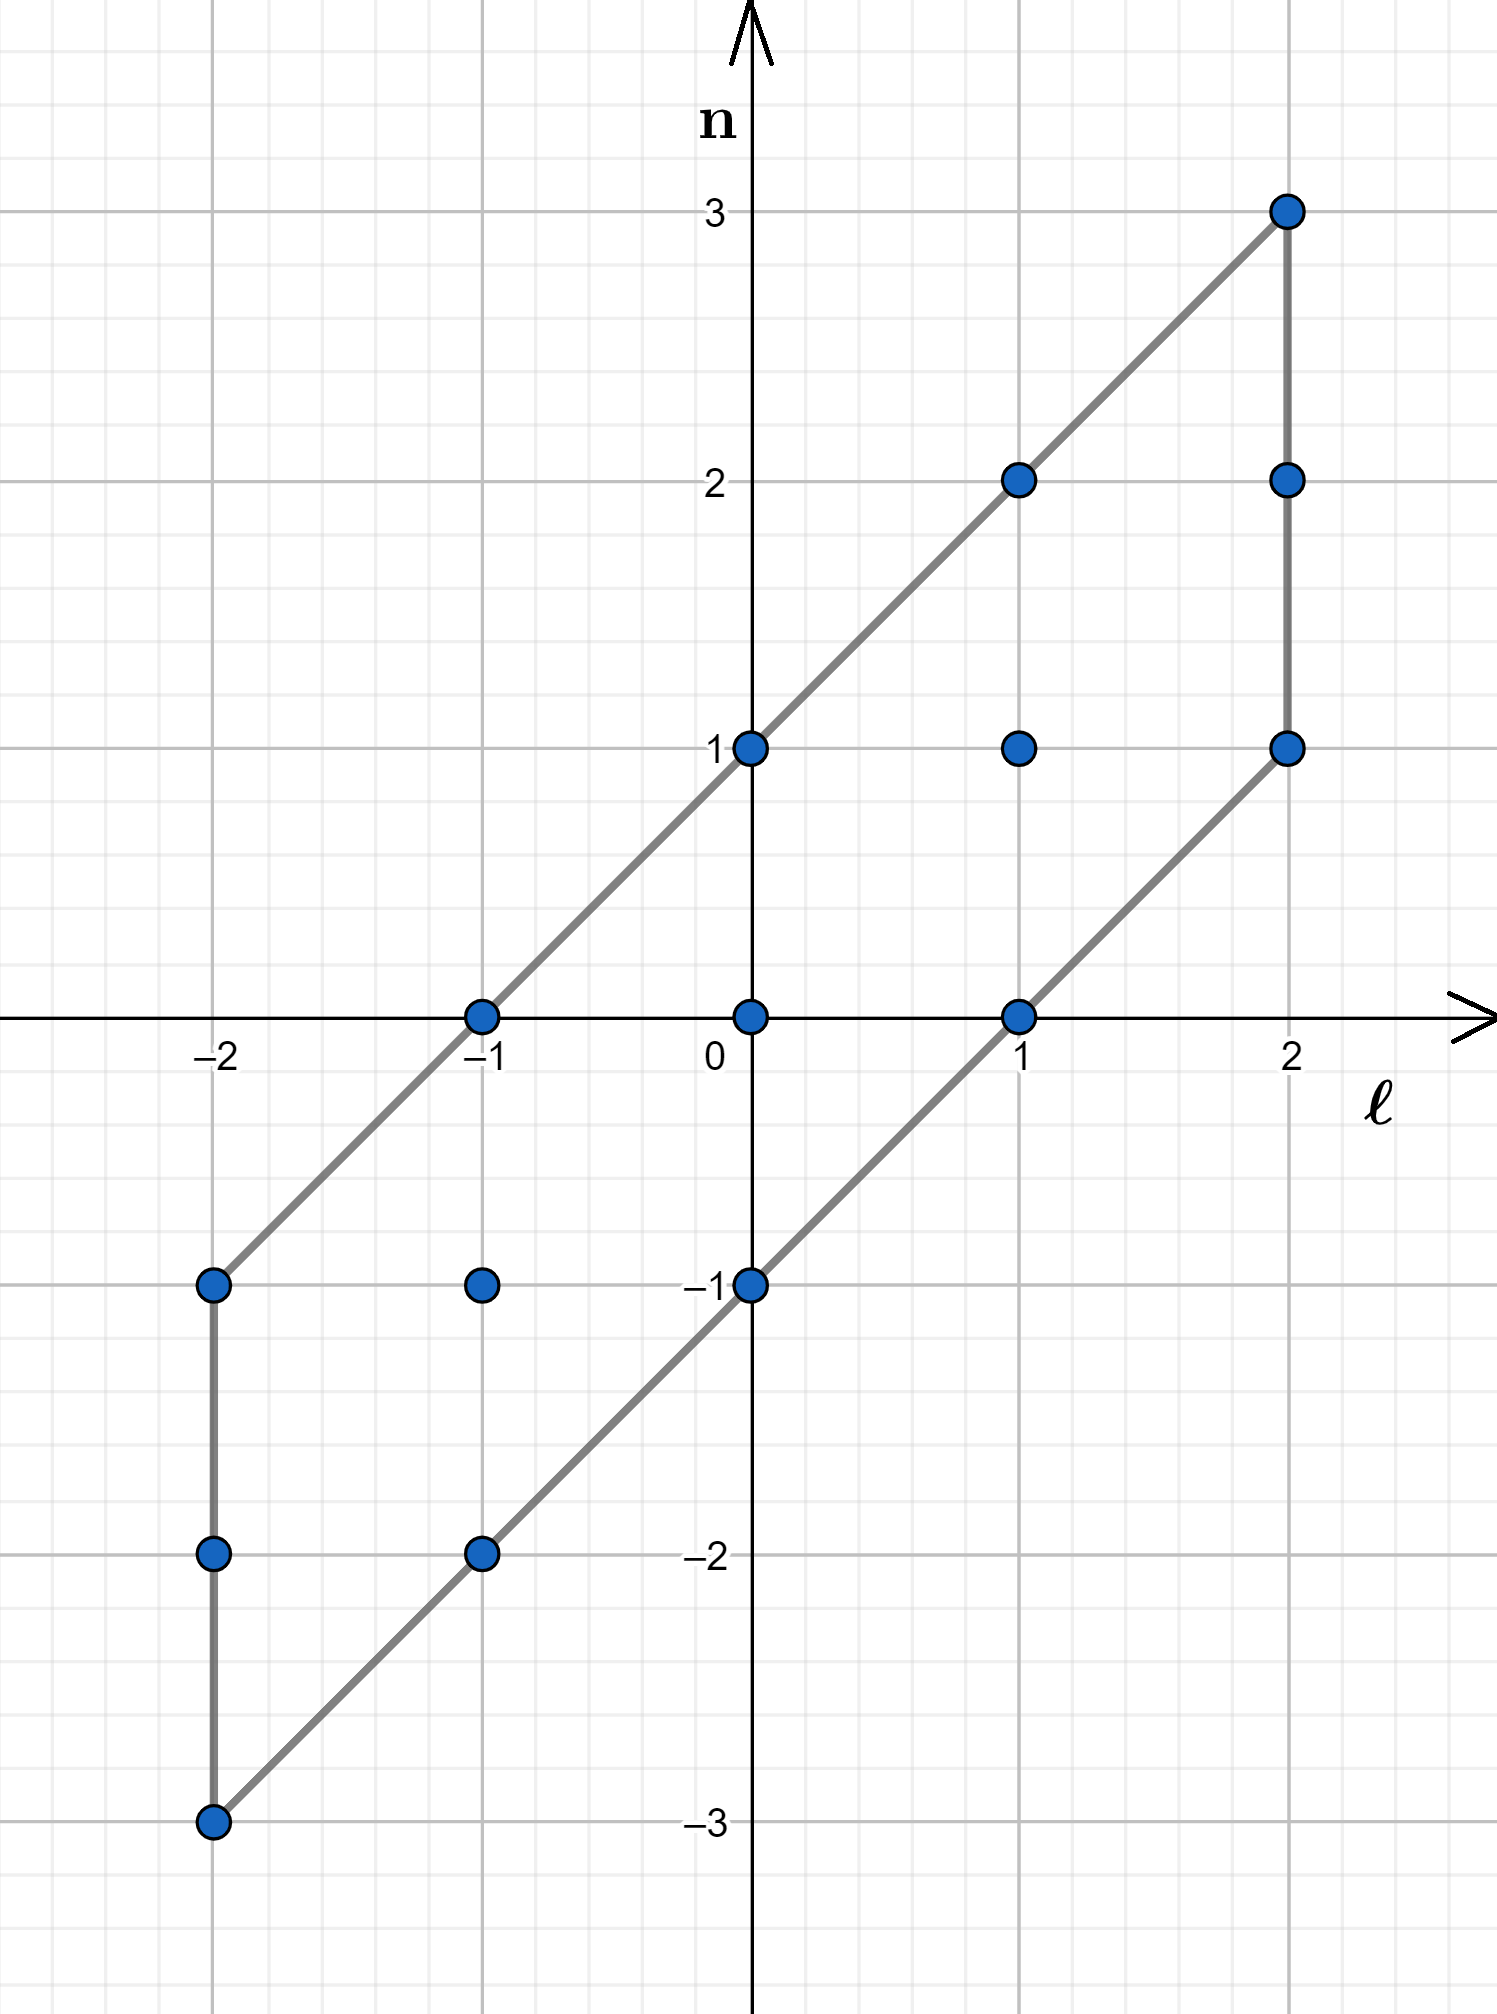
\includegraphics{summArea.png}}
       }
\end{center}
  \caption{Circular case. Summation area for $\ell_{\rm max}=2$ and $Q=1$}
\label{Fig_App_summ}
\end{figure}
%

We start with  $n=N$, for which the sum in Eq.(\ref{xi_n}) reduces to the single term,
$\widetilde\xi_N = \widetilde\alpha_{\ell_{\rm max}} \,\widetilde\sigma_{LL}$
(the upper right corner of the summation area in Fig.\ref{Fig_App_summ}).
This means that the covariance of  $\widetilde B_{Nn}=\Ex\widetilde\xi_N\,\widetilde\xi_n^*$ for any
$n \in [\ell_{\rm max}-Q, \ell_{\rm max}+Q]$ will also contain just one term,
$\widetilde B_{Nn} = \widetilde\sigma_{LL} \, \widetilde\sigma_{\ell_{\rm max},n-\ell_{\rm max}}$
 so that we can restore $\widetilde\sigma_{Lq}$ for all $q$.
First, we note that $\widetilde B_{NN} = |\widetilde\sigma_{LQ}|^2$.
Next, we turn to 
$\widetilde B_{N,\ell_{\rm max}-Q} = \widetilde\sigma_{LQ} \,\widetilde\sigma_{\ell_{\rm max},-Q}^*$
(the lower right corner  of the summation area in Fig.\ref{Fig_App_summ}).
Recalling that 
 $\widetilde\sigma_{\ell, -q} = \widetilde\sigma_{\ell q}^*$, we obtain
$\widetilde B_{N,\ell_{\rm max}-Q}=\widetilde\sigma_{LQ}^2$.
So, from $\widetilde B_{NN} \equiv \widetilde B_{N, \ell_{\rm max}+Q}$ and $\widetilde B_{N,\ell_{\rm max}-Q}$ we know both the modulus 
and the square of the complex number $\widetilde\sigma_{LQ}$, hence it is uniquely
determined. 
By the tight bandwidth assumption (see above in this subsection), 
$\widetilde\sigma_{LQ} \ne 0$, therefore we easily recover  
$\widetilde\sigma_{Lq}$ for all $|q|<Q$ from 
$\widetilde B_{N,\ell_{\rm max}+q} = \widetilde\sigma_{LQ} \,\widetilde\sigma_{Lq}^*$
(the right edge of the 
summation parallelogram in Fig.\ref{Fig_App_summ}).
 
Then, we consider $\widetilde\xi_{N-1}$ and realize that it, again, has just one term,
$\widetilde\alpha_{\ell_{\rm max}-1} \,\widetilde\sigma_{\ell_{\rm max}-1,\ell_{\rm max}-1+Q}$ besides the term that contains 
$\widetilde\sigma_{\ell_{\rm max},\ell_{\rm max}+Q-1}$, which has already been recovered. This allows us to repeat the above process
and uniquely recover $\widetilde\sigma_{\ell_{\rm max}-1,\ell_{\rm max}-1+q}$ for all $q\in[-Q,Q]$. 
And so on, we recover all non-zero $\widetilde\sigma_{\ell q}$,
and therefore all  spectral functions $\sigma_\ell(x)$, from the set of the spectral covariances $\widetilde B_{n \bar n}$.
This completes the proof of uniqueness of the LSM on the circle
provided that
 $\sigma_\ell(x) \ge 0$ 
and the half-bandwidth $Q$ of  $\sigma_\ell(x)$ is such that  $\widetilde\sigma_{\ell Q} \ne 0$ for any $\ell$.




%-------------
\subsection{Spherical case}
\label{App_identif_sphe}




On $\S^2$, the same reasoning is applicable.
We replace the Fourier series in Eq.(\ref{sigma_lq}) by the spherical harmonic
expansion (Laplace series)
%
\begin {equation}
\label{sigma_lqq}
\sigma_\ell(x) = \sum_{q=0}^{Q} \sum_{q'=-q}^{q}     
                          \,\widetilde\sigma_\ell^{qq'} \, Y_{qq'}(x),
\end {equation}
%
where $\widetilde\sigma_\ell^{q,-q'} = (\widetilde\sigma_\ell^{qq'})^*$.
We substitute this expression into Eq.(\ref{LSM}) (where the notation $m$ is changed to $\ell'$):
%
\begin {equation}
\label{LSM_q}
\xi (x) = \sum^{\ell_{\rm max}}_{\ell=0} \sum^\ell_{\ell'=-\ell}  \sum_{q=0}^{Q} \sum_{q'=-q}^{q}     
                          \,\widetilde\sigma_\ell^{qq'}   
                          \,\widetilde\alpha_{\ell \ell'} \, Y_{\ell \ell'} (x) Y_{qq'}(x)
\end {equation}
% 
and project $\xi (x)$ onto $Y_{nn'}(x)$ isolating the spectral component
$\widetilde \xi_{nn'}$ for all $0\le n \le N=\ell_{\rm max}+Q$ and $-n \le n' \le n$. 
The technical difficulty here is that the product  of two spherical harmonics,
 $Y_{\ell \ell'} (x) Y_{qq'}(x)$, when expanded into the 
spherical harmonics basis, yields a number of components (not just one component as 
for the trigonometric series in the circular case above):
%
\begin {equation}
\label{YY}
Y_{\ell \ell'} (x) Y_{qq'}(x) = \sum^{N}_{n=0} \sum^n_{n'=-n} C_{\ell qn}^{\ell'q'n'} Y_{nn'}(x),
\end {equation}
% 
where $C_{\ell qn}^{\ell'q'n'}$ can be expressed using Clebsch-Gordan coefficients 
and is non-zero if and only if 
(i)
the triple $\ell qn$ satisfies the triangle inequality ($|\ell-q|\le n \le \ell +q$),
(ii)
$n'=\ell' + q'$,  and 
(iii) $\ell+q+n$ is an even number \citep[][section 12.9]{Arfken}.

Substituting Eq.(\ref{YY}) into Eq.(\ref{LSM_q}) and utilizing orthogonality
of spherical harmonics, we  write down the expansion 
$\xi(x) =  \sum^{N}_{n=0} \sum^n_{n'=-n} \,\widetilde\xi_{nn'}\,Y_{nn'}(x)$, where
%
\begin {equation}
\label{xi_nn}
\widetilde\xi_{nn'} = \sum C_{\ell qn}^{\ell'q'n'}\,\widetilde\alpha_{\ell\ell'} \,\widetilde\sigma_\ell^{qq'}.
\end {equation}
% 
Here the non-zero terms correspond to the quadruples $\ell,\ell',q,q'$ satisfying
$0\le \ell \le \ell_{\rm max}$,
$0\le q \le Q$,
$|n-\ell|\le q \le n +\ell$,
$\ell+q+n$ is an even number, and
$\ell'+q'=n'$.

Then,  like in the circular case, we start from $\widetilde\xi_{NN}$
and realize that the respective sum in Eq.(\ref{xi_nn}) contains only one term:
$C_{LQN}^{LQN}\,\widetilde\alpha_{LL} \,\widetilde\sigma_L^{QQ}$.
We derive  $\Var \widetilde\xi_{NN}$ and 
$\Cov (\widetilde\xi_{NN},\widetilde\xi_{N,\ell_{\rm max}-Q})$, which allows us to recover  $\widetilde\sigma_L^{QQ}$.
As in the circular case, we assume $\widetilde\sigma_L^{QQ} \ne 0$.
This allows us to recover all $\widetilde\sigma_L^{Qq'}$ by 
computing $\Cov (\widetilde\xi_{NN},\widetilde\xi_{N,\ell_{\rm max}+q'})$ for all $-Q \le q' \le Q$.


After that, we compute $\Cov (\widetilde\xi_{NN},\widetilde\xi_{N-1,\ell_{\rm max}-1+q'})$ for all $-Q \le q' \le Q$,
retrieving  $\widetilde\sigma_L^{Q-1,q'}$. Proceeding in this way for $n=N-2, N-3,\dots$, 
we recover all $\widetilde\sigma_L^{qq'}$.
Knowing $\widetilde\sigma_L^{qq'}$, we can repeat the above process to recover 
 $\widetilde\sigma_{\ell_{\rm max}-1}^{qq'}$, and so on, until all $\widetilde\sigma_\ell^{qq'}$ are found.

So, we have shown that all  $\widetilde\sigma_\ell^{qq'}$ and thus all  $\sigma_\ell(x)$
can be uniquely determined from the process (spectral) covariances.
This proves the uniqueness of the LSM in the spherical case whenever 
$\sigma_\ell(x) \ge 0$ 
and the half-bandwidth $Q$ of the process $\sigma_\ell(x)$ is such that  $\widetilde\sigma_\ell^{QQ} \ne 0$ 
 for any $\ell$.







%-------------
\section {Spectral loss function}
\label{app_specLoss}



Here we derive an {\em analysis-error related} loss function to train the neural network 
that extracts the local spectrum from the local band variances.
Devising such a targeted loss function was crucial for the success of the neural network based approach.

We set up a hypothetical simplified linear analysis and look at the analysis error variance.
We consider, first, the (mean-square) optimal analysis, which has access to the  {\em true background-error}
(forecast-error)
covariances. Second, we consider the same analysis but with  {\em misspecified background 
error} covariances (the suboptimal analysis). 
Both analyses have access to the true {\em observation-error} covariances.
We define the loss function to be the {\em excess of the suboptimal-analysis error variance
over that of the optimal analysis}.

Specifically, on the unit sphere, let the forecast-error field, $\xi(x)$, be zero-mean, stationary, band-limited 
(with the maximum wavenumber $\ell_{\rm max}$ so that it can be represented on an  analysis grid),
and have the spectrum $f_\ell$.
Let the observations $X^{\rm obs}_i$ be located at every analysis grid point
(so that $X^{\rm obs}$ can be viewed as a spatial field) and
have independent zero-mean errors $\eta_i$ all
with the same variance. 
Finally, assume, for simplicity, that the analysis background is zero.

Since both $\xi$ and $\eta$ are stationary (isotropic on the sphere), 
their spectral-space covariance matrices are diagonal. Therefore, the simplified
analysis decouples into a series of partial analyses performed for each wavenumber pair $(\ell,m)$
separately and independently.

For each partial analysis, by $X^{\rm true}_{\ell m} = -\xi_{\ell m}$ denote the projection of the truth
$X^{\rm true}(x)$
on $Y_{\ell m}$ (recall that the background is postulated to be equal to zero) and
by $X^{\rm obs}_{\ell m} = X^{\rm true}_{\ell m} + \eta_{\ell m} = \eta_{\ell m} - \xi_{\ell m}$
the respective projection of the observation field.
The optimal estimate of the truth (\ie the optimal analysis) in spectral space will then be
%
\begin {equation}
\label{XaOpt}
X^{\rm a}_{\ell m} = K_\ell X^{\rm obs}_{\ell m} = K_\ell (\eta_{\ell m} - \xi_{\ell m}),
\end {equation}
%
where
%%
%\begin {equation}
%\label{Kl}
$K_\ell = \frac{f_\ell}{f_\ell + r}$
%\end {equation}
%
is the optimal-analysis gain and 
$r$ is the spectral-space observation error variance (which is constant since $\eta(x)$ is 
the band-limited white noise by construction). 
With the misspecified analysis, we assume that the gain is defined with the
misspecified $f_\ell'$ instead of the true $f_\ell$, that is, 
$K_\ell' = \frac{f'_\ell}{f'_\ell + r}$.

Then, for the sub-optimal $K_\ell'$, the analysis error is  
$\delta X^{\rm a}_{\ell m} = X^{\rm a}_{\ell m} +\xi_{\ell m} = (1-K_\ell')\xi_{\ell m} +  K_\ell' \eta_{\ell m}$.
Its variance is
%
\begin {equation}
\label{dXa}
A_\ell := \Var \delta X^{\rm a}_{\ell m}= 
  \frac{r^2 f_\ell}{(f_\ell' + r)^2} + \frac{(f'_\ell)^2 r}{(f_\ell' + r)^2}.
\end {equation}
%
Its excess over the optimal-analysis error variance is then
%
\begin {equation}
\label{dXa2}
\Delta A_\ell =  \frac{r^2 f_\ell}{(f_\ell' + r)^2} + \frac{(f'_\ell)^2 r}{(f_\ell' + r)^2} - 
                 \frac{r^2 f_\ell}{(f_\ell + r)^2}  - \frac{(f_\ell)^2  r}{(f_\ell  + r)^2}.
\end {equation}
%
Summing all spectral-space contributions, we obtain the loss function 
%
\begin {equation}
\label{loss_S2}
{\cal L}({\bf f, f}') := \sum_{\ell=0}^{\ell_{\rm max}} \frac{2\ell +1}{4\pi} \Delta A_\ell =  
  r^2 \sum_{\ell=0}^{\ell_{\rm max}}\frac{2\ell +1}{4\pi} \frac{(f'_\ell - f_\ell)^2}{(f_\ell  + r) (f'_\ell  + r)^2}.
\end {equation}
%
Here ${\bf f, f}'$ are the vectors comprised by all spectral variances
$f_\ell$ and $f_\ell'$, respectively.
Note that the resulting loss function Eq.(\ref{loss_S2}) is not a norm, it is rather a {\em deviance}, that is,
${\cal L}({\bf f, f}') \ge 0$  and ${\cal L}({\bf f, f}') = 0$ if and only if ${\bf f = f}'$.

On the circle, the setup and the derivation are the same (omitted). The expression for the 
loss function differs from Eq.(\ref{loss_S2}) only in the absence of the factor 
$\frac{2\ell +1}{4\pi}$ and in the summation range (from $-\ell_{\rm max}+1$ to $\ell_{\rm max}$).







%-----------------------------
\section{Consistency of the estimator of band variances}
\label{App_consist}



Here we consider  bandpass filtering of a locally stationary process
and find conditions under which the approximations Eqs.(\ref{xi_j}) and (\ref{vj2}) hold.
For simplicity, we examine the circular case.

Let the linear filter ${\cal H}$ with the spectral transfer function $H(\ell)$ be applied
to the locally stationary 
process 
%
\begin {equation}
\label{LSM_S1_}
\xi (x) =  \sum_{\ell=-\ell_{\rm max}}^{\ell_{\rm max}}  \sigma_\ell(x)  
                          \,\widetilde\alpha_{l} \, \e^{\i \ell x}
\end {equation}
%
(we reproduce here our basic Eq.(\ref{LSM_S1}) for the reader's convenience).
In spectral space, the action of a linear filter on the signal
$\xi (x) = \sum_\ell   \widetilde\xi_\ell \,\e^{\i \ell x},$ amounts to the 
multiplication of spectral coefficients $\widetilde\xi_\ell$ by the respective $H(\ell)$.
The spectral-space representation of $\xi(x)$ is given by Eq.(\ref{xi_ln}) so that
the filtered process $\xi_{\cal H} = {\cal H}\xi$ reads
%
\begin {equation}
\label{xi_H}
\xi_{\cal H} (x) =  \sum_{\ell=-\ell_{\rm max}}^{\ell_{\rm max}} \widetilde\alpha_{\ell} \, \e^{\i \ell x} 
           \sum_{q=-Q}^{Q} H(\ell+q) \,\widetilde\sigma_{\ell q} \, \e^{\i  q x}.
\end {equation}
%
Now we recall that the local stationarity means that the processes $\sigma_\ell(x)$ 
are slowly changing in space (\ie with $x$), which is equivalent to a  rapid decrease of the 
coefficients $\widetilde\sigma_{\ell q}$ in 
their spectral decomposition 
$\sigma_\ell(x) = \sum_q  \widetilde\sigma_{\ell q} \, \e^{\i  q x}$ 
(Eq.(\ref{sigma_lq})) for any wavenumber $\ell$. 
If  we specify  $H(\ell)$ to change  with $\ell$ much more slowly than $ \widetilde\sigma_{\ell q}$
change with $q$, then,
in the sum over $q$ in Eq.(\ref{xi_H}),  $H(\ell+q)$ 
can be approximated by  $H(\ell)$ leading to the approximation
%
\begin {equation}
\label{LSM_S1_H}
\check\xi_{\cal H} (x) =  \sum  \sigma_\ell(x)  
                          \,\widetilde\alpha_{l} \, H(l) \,\e^{\i \ell x}.
\end {equation}
%
(Its spherical counterpart is given in Eq.(\ref{xi_j}).)
A more rigorous proof of this statement follows.
The error in the approximation Eq.(\ref{LSM_S1_H}) is
%
\begin {equation}
\label{LSM_S1_H_err}
\check\xi_{\cal H} (x)  - \xi_{\cal H} (x) =  
   \sum_{\ell} \widetilde\alpha_{\ell} \, \e^{\i \ell x} 
   \sum_{q} \left[ H(\ell+q) - H(\ell) \right] \,\widetilde\sigma_{\ell q} \, \e^{\i  q x},
\end {equation}
%
Here we remember that ${\cal H}$ is a bandpass filter and assume that its 
spectral transfer function is generated by a bell-shaped function of continuous argument, $\kappa(z)$, such that
$\kappa(0)=1$ and a  half-width of $\kappa(z)$ is also about 1.
%(more precisely, we require that $\max|\kappa'(z)| = 1$).
Specifically, let
%
\begin {equation}
\label{H_kappa}
H(\ell) = \kappa \left(\frac{\ell-\ell^{\rm c}}{d} \right),
\end {equation}
%
where $\ell^{\rm c}$ is the band's central wavenumber and $d$ is the half-bandwidth
(\cf Eq.(\ref{Hj})).
As we noted above, since $\widetilde\sigma_{\ell q}$ rapidly decays with the growing $|q|$ for any $\ell$, 
the use of the first order Taylor series approximation is warranted:
$H(\ell+q) \approx H(\ell) + H'(\ell)q = H(\ell) + \kappa'(.) q/d$.
Substituting this equation into Eq.(\ref{LSM_S1_H_err}) yields
% and utilize Eq.(\ref{H_kappa}):
\begin {equation}
\label{LSM_S1_H_kappa}
\check\xi_{\cal H} (x)  - \xi_{\cal H} (x) =  \frac{1}{d}
   \sum_{\ell}  \widetilde\alpha_{\ell} \, \e^{\i \ell x}  \kappa'(.)
   \sum_{q} q \,\widetilde\sigma_{\ell q} \, \e^{\i  q x} \equiv
   \frac{1}{\i d} \sum_{\ell}  \widetilde\alpha_{\ell} \, \e^{\i \ell x}  \kappa'(.) \sigma_\ell'(x)
\end {equation}
%
(the second equality is due to  
$\sigma_\ell'(x) = \sum_{q}  \i q \,\widetilde\sigma_{\ell q} \, \e^{\i  q x}$).

Next, we compute the mean square value of Eq.(\ref{LSM_S1_H_kappa})
and note that the width $d$ of the spectral transfer function $H(\ell)$ equals the inverse width $L_{\rm H}$
of the impulse response function of the filter $h(x)$ (which is the inverse Fourier transform of $H(\ell)$),
getting
%
\begin {equation}
\label{LSM_S1_H_kappa_var}
\Ex\left( \check\xi_{\cal H} (x)  - \xi_{\cal H} (x)  \right)^2 = L_{\rm H}^2
   \sum_{\ell}  (\kappa'(.) \,\sigma_\ell'(x))^2.
%   \le  L_{\rm H}^2 \sum_{\ell} (\sigma_\ell'(x))^2 .
\end {equation}
%
With
%
\begin {equation}
\label{sigma_ell}
\sigma_\ell(x) =\sum_q  \phi_\ell(qT) \, \e^{\i  q x}
\end {equation}
%
(see Eqs.(\ref{vlq}) and  (\ref{sigma_lq}),
%
\begin {equation}
\label{sigma_ell_prim}
|\sigma_\ell'(x)| \le  \sum_q  |q| \,  |\phi_\ell(qT)|.
\end {equation}
%
Since $ \kappa'(.) = O(1)$ and the range of both $\ell$ in Eq.(\ref{LSM_S1_H_kappa_var})
and $q$ in Eq.(\ref{sigma_ell}) are finite, the asymptotics Eq.(\ref{phiT})
implies that 
$\Ex\left( \check\xi_{\cal H} (x)  - \xi_{\cal H} (x)  \right)^2$
as 
$T \to \infty$.

So, indeed, the mean-square error in the approximation Eq.(\ref{LSM_S1_H})
is asymptotically zero in the limit of local stationarity.



QQ
In practical terms, for small approximation error, the width of the filter's impulse response function $L_{\rm H}$ is required
to be much shorter than the non-stationarity length scale $\Lambda$.
This is conceivable because at intervals shorter than  $\Lambda$, the LSM process 
behaves like a stationary process.

The above result implies that
with the norm defined from $\| . \|^2 := \Ex (.)^2  $,
we have $\| \check\xi_{\cal H} - \xi_{\cal H} \| \to 0$.
Therefore, $\| \check\xi_{\cal H}\|^2 \to \|\xi_{\cal H} \|^2$
so that the approximate band variance estimate
$ \sum  H^2(l) \sigma_\ell^2(x)$
% (see Eq.(\ref{vj2})), which follows from
%Eq.(\ref{LSM_S1_H}) 
is asymptotically unbiased and consistent.


Spherical case...QQ



%-----------------------------------------

\bibliography{mybibfile}

%-----------------------------------------

\end{document}
